\documentclass[a4paper,leqno]{article}

\usepackage[T1]{fontenc}
\usepackage[utf8]{inputenc}
\usepackage[english]{babel}
\usepackage{amsmath}
\usepackage{longtable} 
\usepackage{multirow} 
\usepackage{graphicx}
\usepackage{algorithm2e}
\usepackage{listings}
\usepackage{caption}


\begin{document}
	
	
	\date{2017/11/26}
	\author{Bolshakova Liubov\\ Campagnoli Chiara\\ Lagni Luca}
	\title{\textbf{\huge Travlendar+}\\ Design Document}
	\begin{minipage}[!t]{\linewidth}
		\centering
		
\includegraphics[scale=0.8]{logo2}
	\end{minipage}
	\begin{minipage}[!h]{\linewidth}
		\maketitle 
	\end{minipage}
	
	\newpage
	\tableofcontents                        
  
\newpage	
\section{Introduction}

\subsection{Purpose}
The purpose of this document is to provide information about the design decisions we made for the development of the system Travlendar+. More in detail, it includes an overview about architectural design, description and interactions of the main components of the system, some possible design patterns that can be used for implementation, the description of some of the main algorithms and the plan of implementation, integration and test. It is mainly addressed to the developers of the system.

\subsection{Scope}
Travlendar+ is a calendar based applications, which allows the user to create meetings with different locations and computes the best way to reach such locations. It includes different means of tansport, both public and personal, autonomous and not. Amonng its functionalities there are the possibility of creating flexible breaks between meetings, deselecting travel means the user does not wish to use and choosing the combination of travel means which minimizes the carbon footprint. Besides, it supports the user in the reservation of cars and bikes of a vehicle-sharing service and in the purchase of tickets of public transport companies.\\
More details about the goals and functionalities of the system can be found in the RASD.

\subsection{Definitions, Acronyms, Abbreviations}
\begin{itemize}
	\item API: Application Programming Interface.
	\item DD: Design Document
	\item GPS: Global Positioning System.
	\item GSM: Global System for Mobile Communications.
	\item GUI: Graphical User Interface.
	\item OAMOT: Other Autonomous Means of Transport
	\item ONAMOT: Other Non-Autonomous Means of Transport
	\item OS: Operating System.
	\item RAM: Random-access memory.
	\item RASD: Requirement analysis and Specification Document.
	\item SMS: Short Message Service.
\end{itemize}

%\subsection{Revision history}

\subsection{Reference Documents}
\begin{itemize}
	\item Mandatory Project Assignments.pdf
	\item Requirements Analysis and Specification Document
	\item Design Deliverable Sample from A.Y. 2015-2016.pdf
	\item DD From the car sharing project.pdf
	\item Integration and test plan from the car sharing project.pdf
\end{itemize}

\subsection{Document Structure}
Besides the introduction, the document is divided into five main parts:
\begin{enumerate}
	\item Architectural design: it contains all the main decisions about the general architecture of the system. In particular, here is specified the tier division of the proposed system and are included the main diagrams (component diagrams, deployment diagrams, runtime diagrams and the complete class diagram). Here are also described some of the possible design patterns which can be used for implementation.
	\item Algorithm design: it includes a description of some of the main algorithms that will be used to implement our system.
	\item User interface design: it inludes some mockups of the mobile application interface, undelying how the main functionalities of the system can be accessed by the user.
	\item Requirements traceability: it explains how the requirements identified in the RASD have been fullfilled in the design elements and decisions.
	\item Implementation, integration and test plan: it explains the order in which we are going to implement, integrate and test the components of the system.
\end{enumerate}

\newpage
\section{Architectural design}

\subsection{Overview}
Travlendar+ is based on a three-tier architecture. A diagram of the proposed system was already present in section 2.4.3 of the RASD; here we provide on the same diagram a division between the different tiers and a more detailed description of each one of these.

\begin{figure}[!h]
	\begin{centering}
		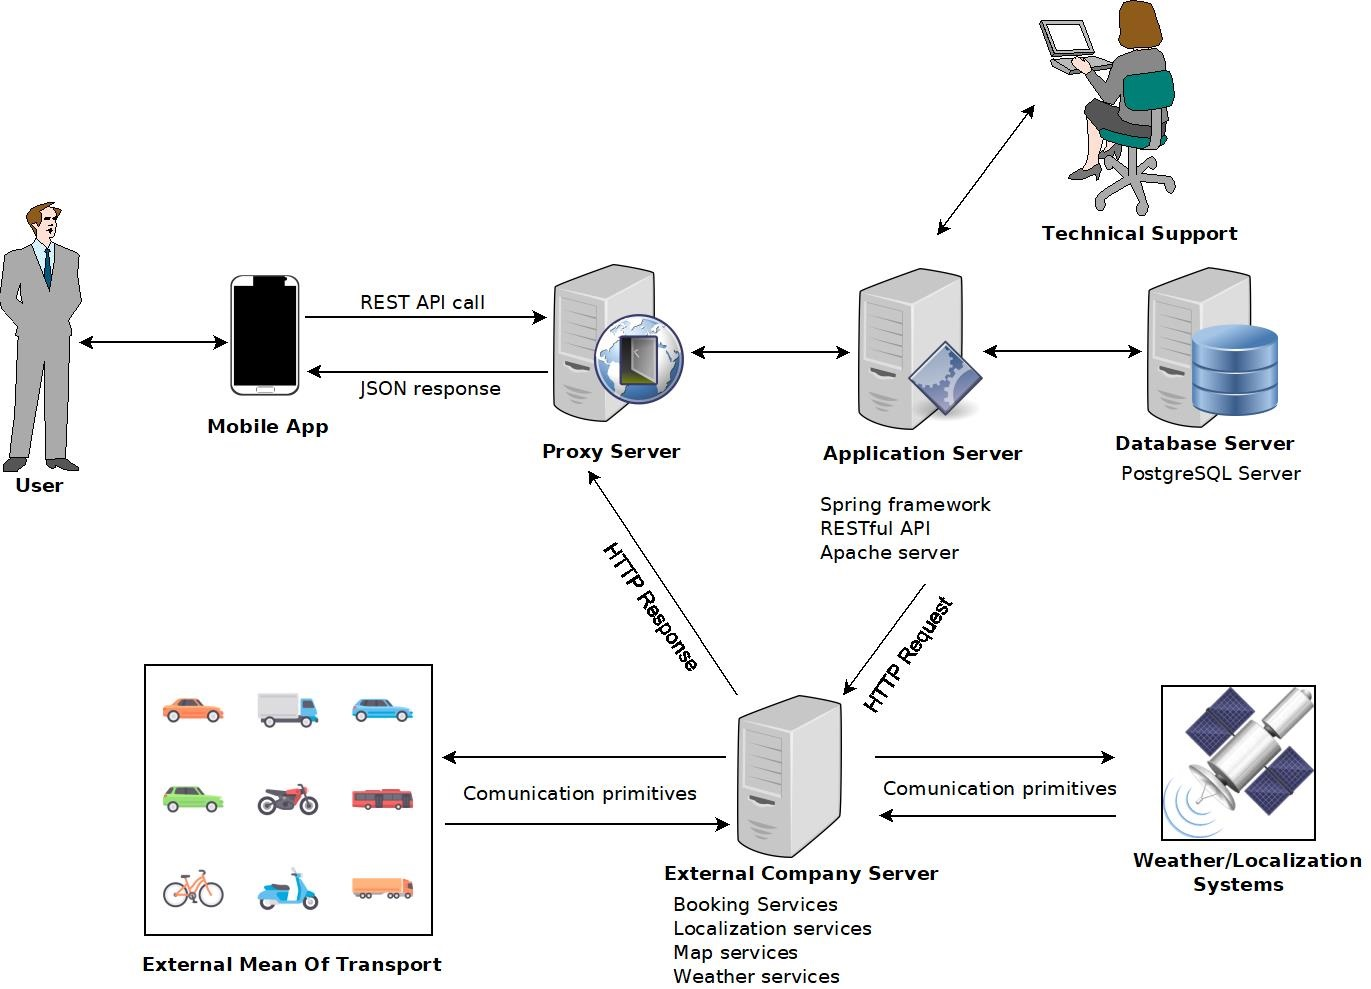
\includegraphics[scale=0.3]{ProposedSystemDiagram_29102017_1}
	\end{centering}
	\caption{Proposed system with tier division. Red: presentation, Blue: logic, Green: data}
\end{figure}

The presentation layer consists of the mobile application, which provides a GUI for the interaction of the user with the service.\\
The logic layer is mainly represented by the application server, where all main decisions and computation take place, although a small part of logic is left to the mobile application (simple elaborations of data such as the location of the user through GPS, or remodeling of the view presented to the user).\\
A proxy server is inserted between the application server and the mobile application for security reasons.\\
Finally, the data layer is represented by the database server, interacting with the application server when needed.

\newpage
\subsection{Component view}
From a high level point of view, the system is composed by three elements: the user, the server and the database. The user, which can be in general registered or unregistered, interacts with the server through the mobile application. On the server side, the application is the component which takes care of performing most of the system's functionalities. After the user has performed a request, he has to wait for the server's response whether it was successful or not. The technical support application is the component of the server dedicated to the technical support staff, which is responsible of fixing problems such as providing new links of external companies in case of broken ones. The information about registered users are stored in the database; the user doesn't directly communicate with the database, but always through the server.
\begin{figure}[!h]
	\centering
	\begin{center}
		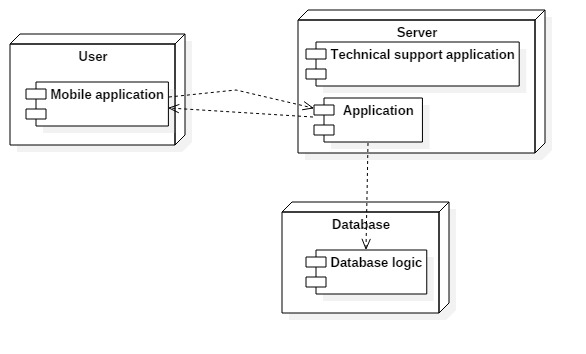
\includegraphics[scale=0.3]{ComponentHighView_241117_1}
	\end{center}
	\caption{High level component diagram}
\end{figure}

From a more detailed point of view, the application on server is made of different components, each one taking care of different functionalities:
\begin{itemize}
	\item Push Gateway: device for sending push notification to the user
	\item MeetingNotifier: is responsible for communication with the user device (notification of upcoming meeting)
	\item Router: handles the incoming data, sorting it to the right controller
	\item ECManager: component containing all the procedures to manage communication with external companies and retrieve all the needed information from them
	\item MeetingBuilder: component that is responsible of creating meetings and breaks and managing the schedule of the user
	\item TripBuilder: component that is responsible of computing trips based on the information retrieved from the ECManager
	\item LoginController: component that controls the registration of clients and their access 
	\item ProfileManager: component that manages the information related to a client (operations such as the setting and change of saved preferences)
	\item InfoProvider: provides access to static information about the system, such as rules and contacts for assistence
\end{itemize}

\begin{figure}[!h]
	\centering
	\begin{center}
		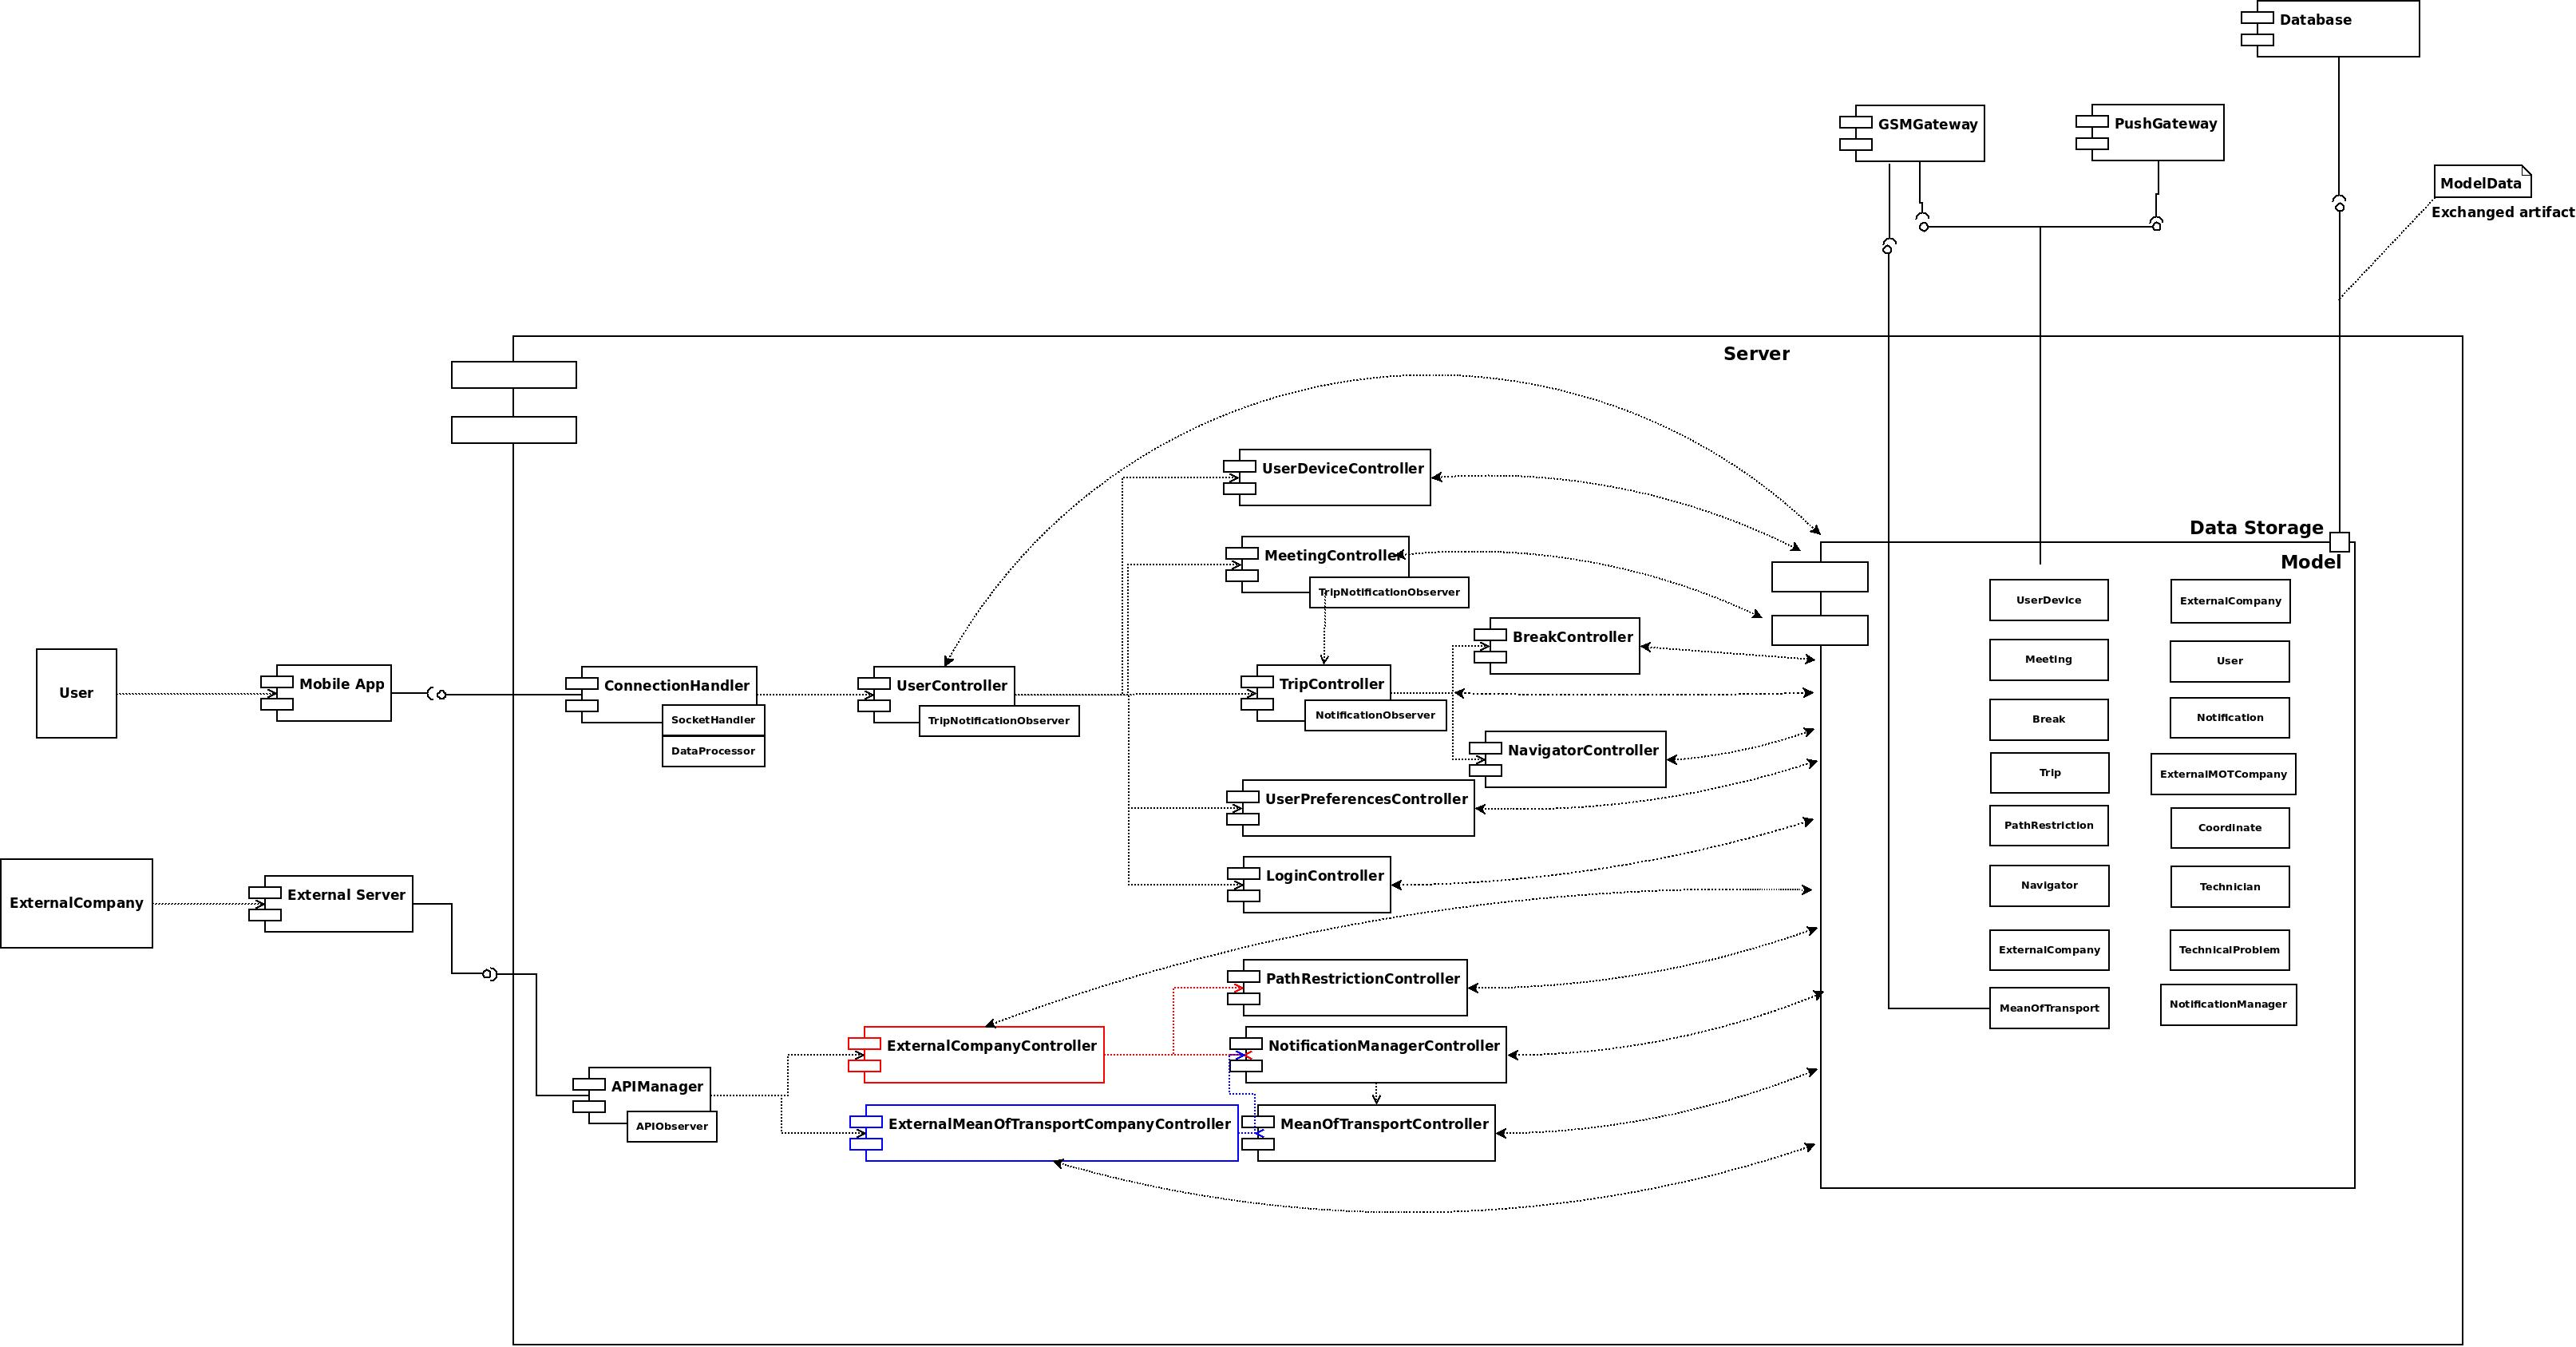
\includegraphics[scale=0.15, angle = 90]{UMLComponentView_24112017_2}
	\end{center}
	\caption{More detailed component diagram}
\end{figure}

\newpage
\subsection{Deployment view}
\begin{figure}[!h]
	\centering
	\begin{center}
		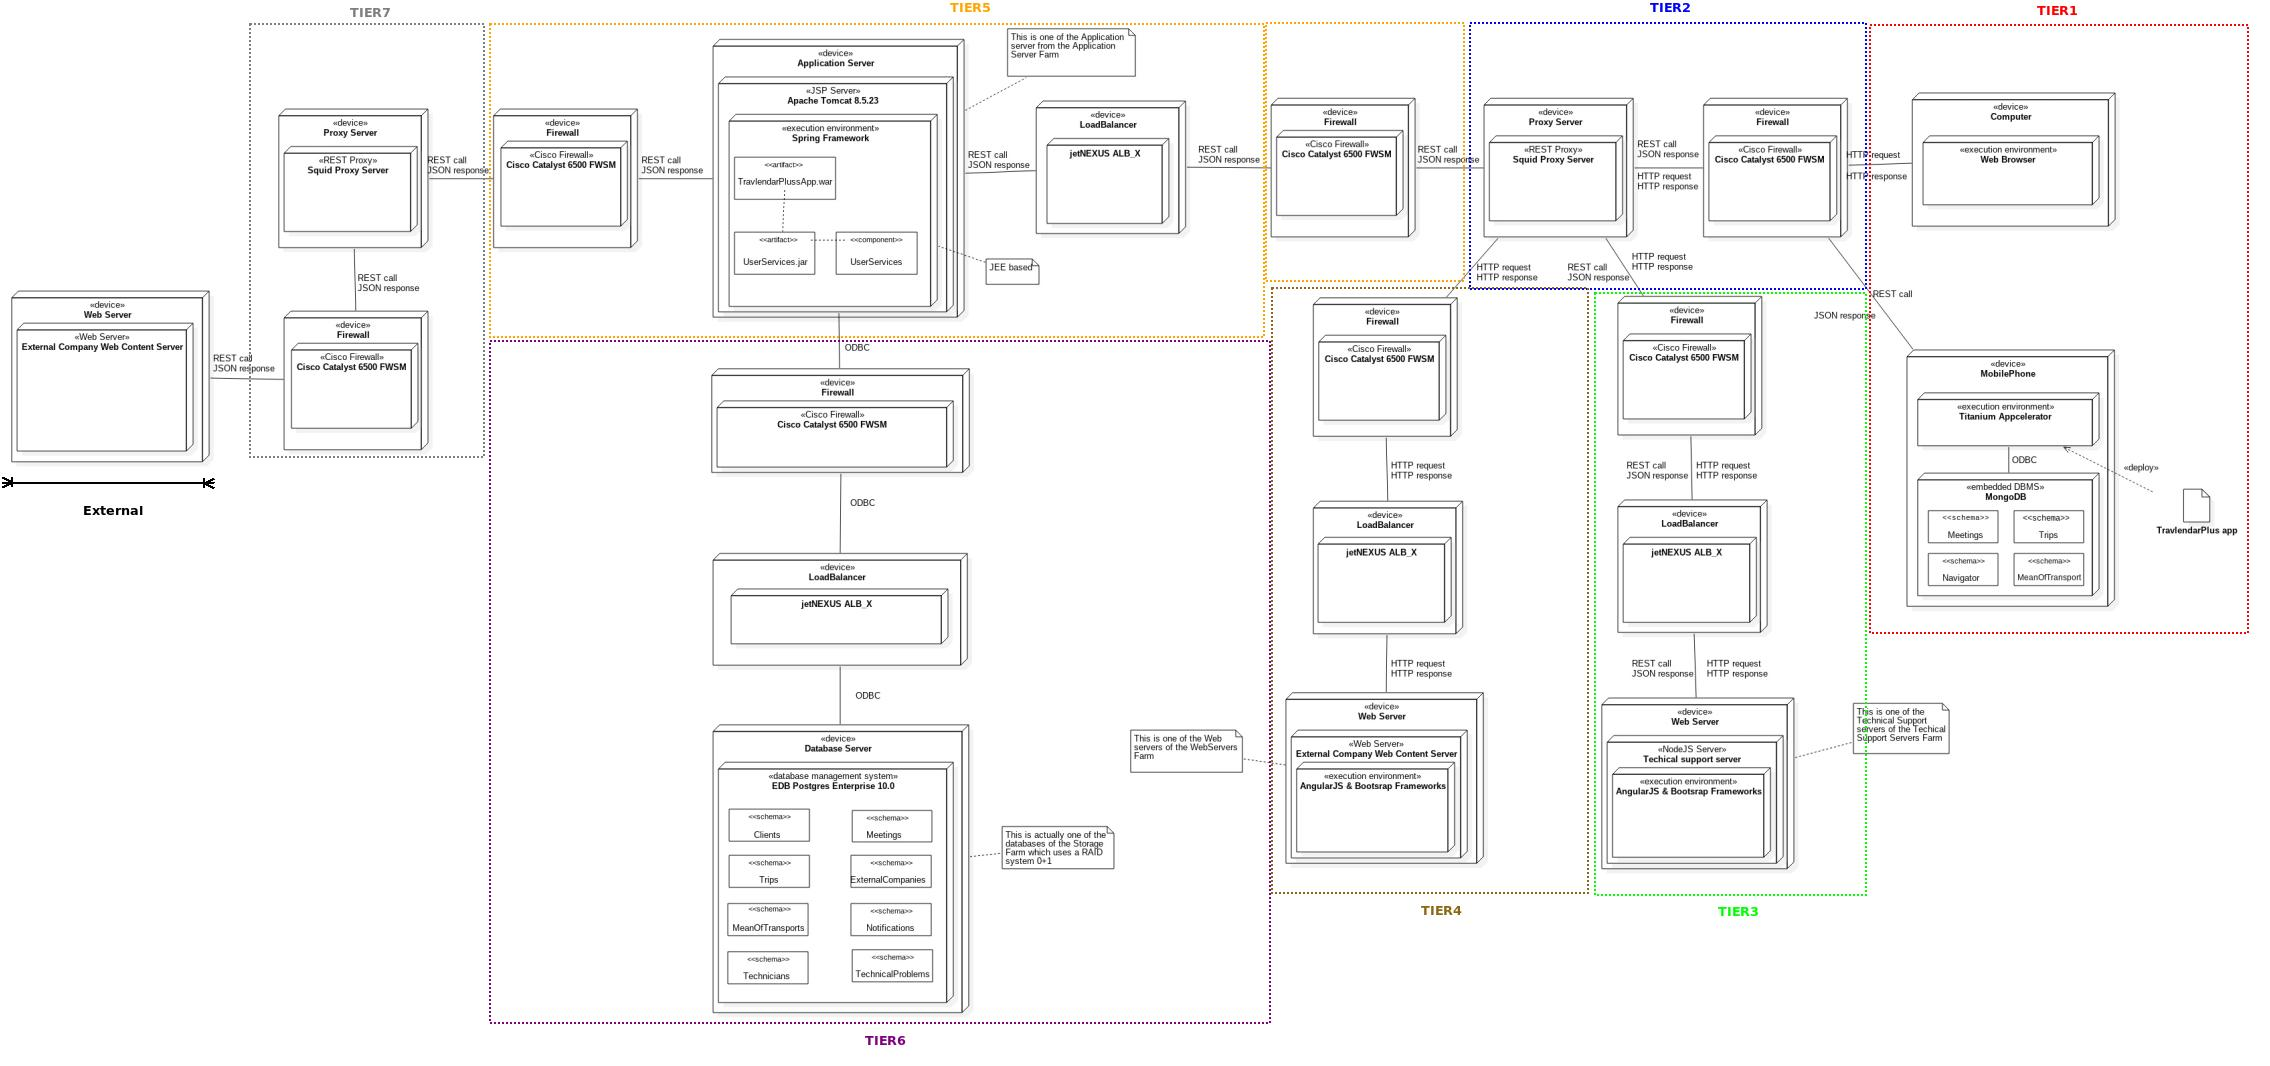
\includegraphics[scale=0.225, angle = 90]{TravlendarPlusDeploymentDiagramTiers_19112017_1}
	\end{center}
       \caption{Deployment diagram}
\end{figure}


\newpage
\subsection{Runtime view}

\subsubsection{Meeting creation}

\begin{figure}[!h]
	\centering
	\begin{center}
		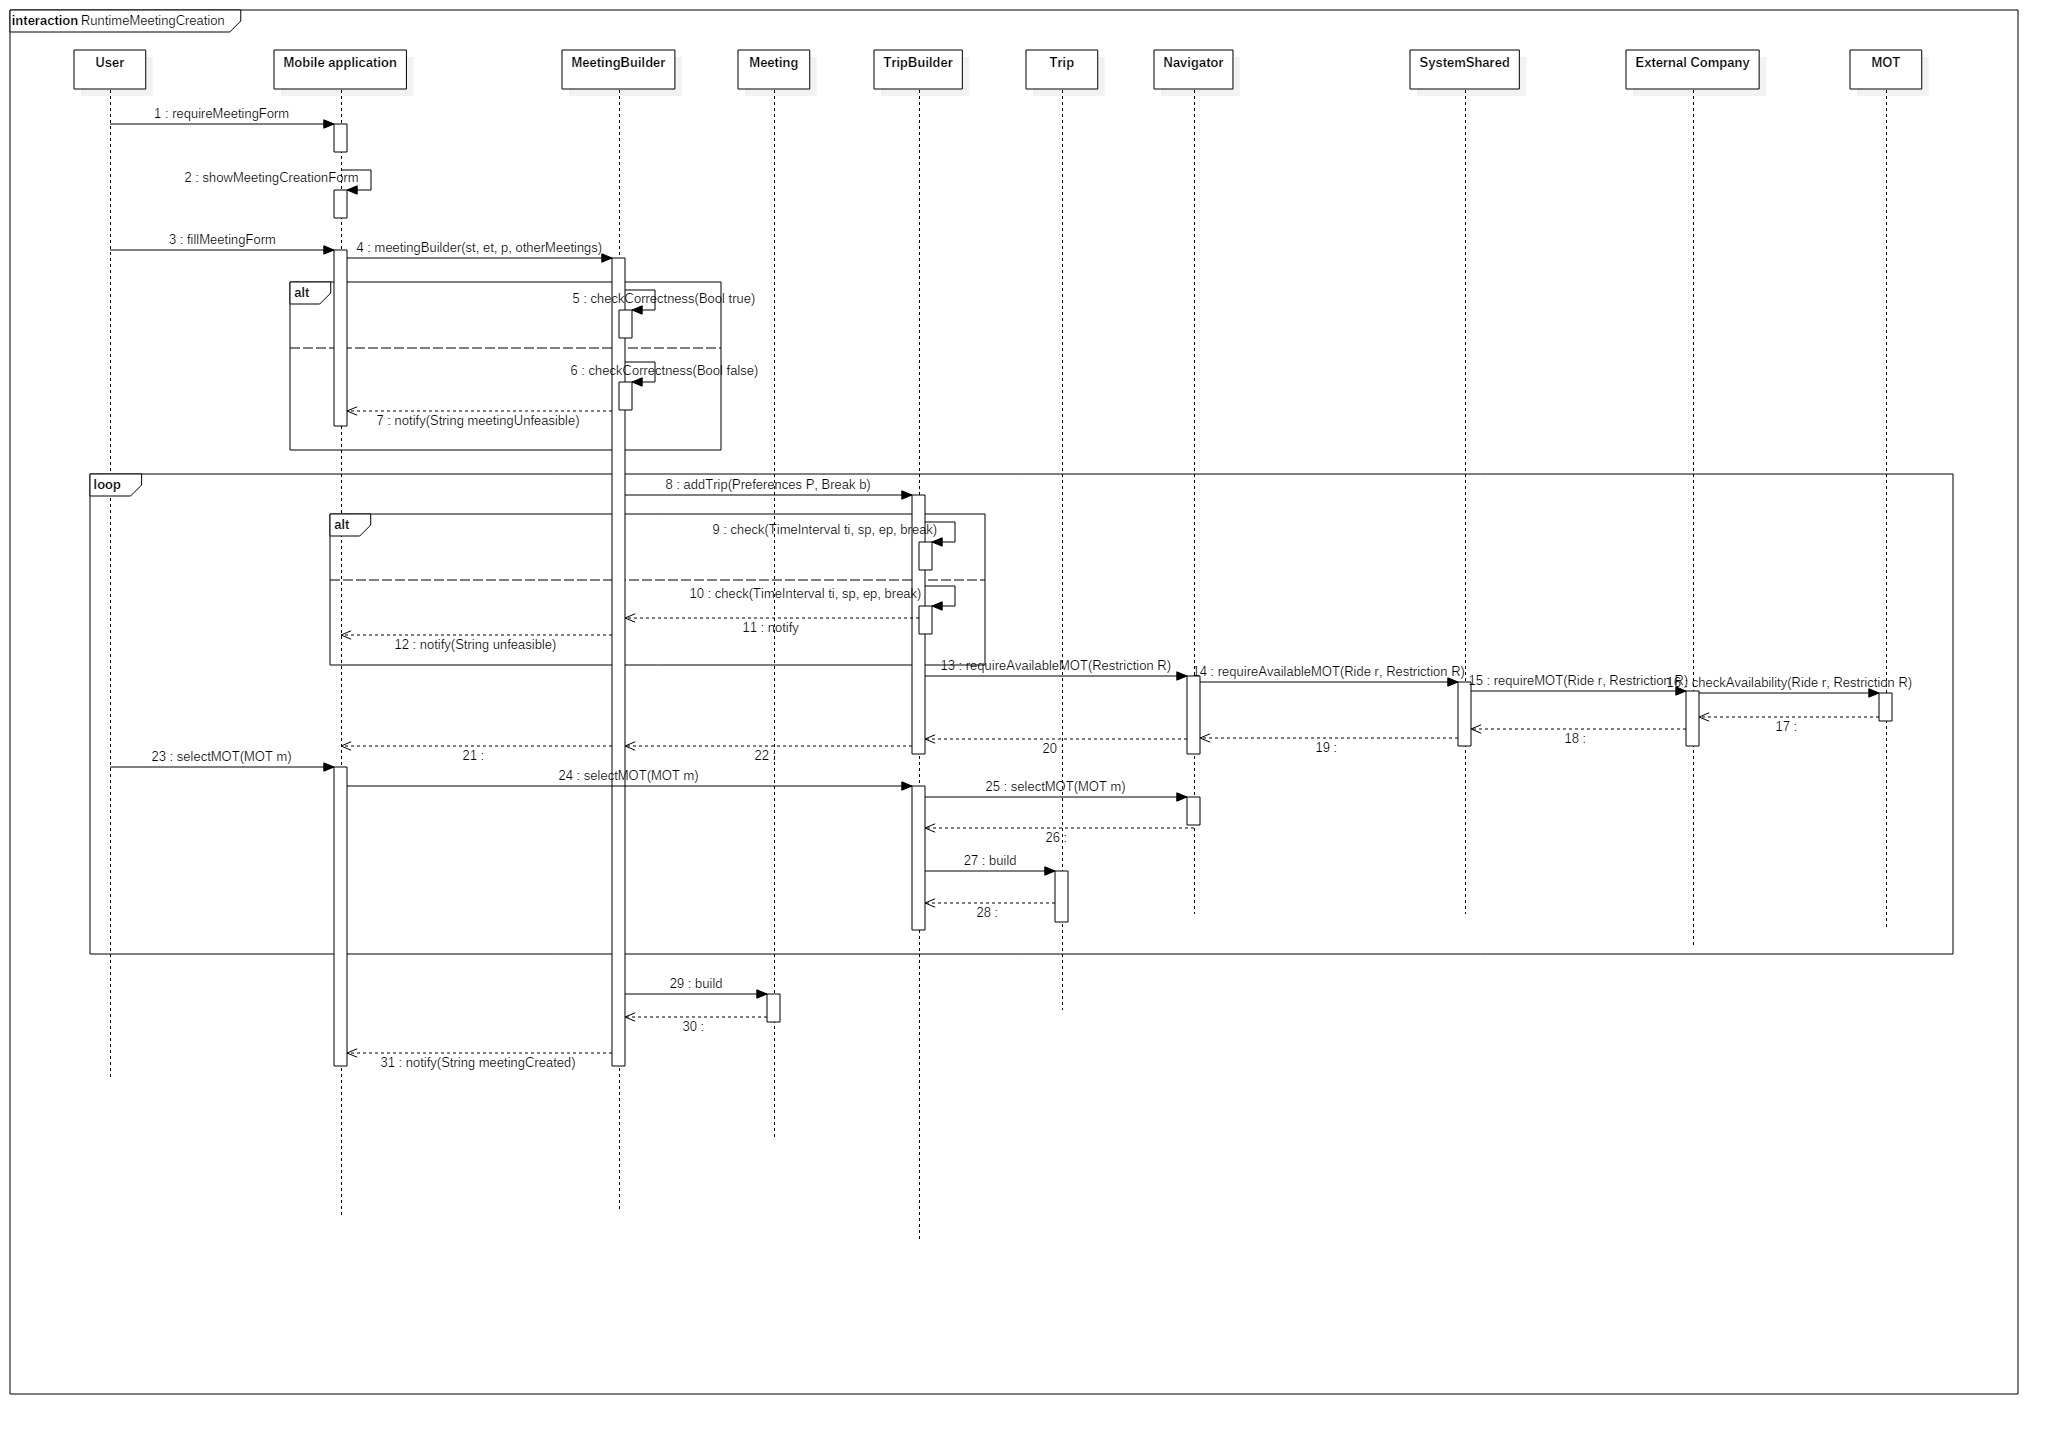
\includegraphics[scale=0.2, angle = 90]{RuntimeMeetingCreation_191117_1}
	\end{center}
	\caption{Runtime sequence diagram of meeting creation}
\end{figure}

This sequence diagram describes the runtime interaction between the components during the creation of a meeting. It refers to use cases 3, 4, 5, 17, 18, 19 and 21 described in section 3.2.2 of the RASD.\\
We illustrated the more general case in which the user is a visitor, that means
an unregistered user: this means that he or she is asked to insert his preferences and constraints (for example deselect unwanted travel means or choice of the most ecological
route) as inputs for the meeting creation. The only difference with a client, or registered user, is that these settings may have been saved, if the user has chosen to,
and they will be searched for in the database.


\subsubsection{Vehicle sharing reservation and ticket purchase}


\begin{figure}[!h]
	\centering
	\begin{center}
		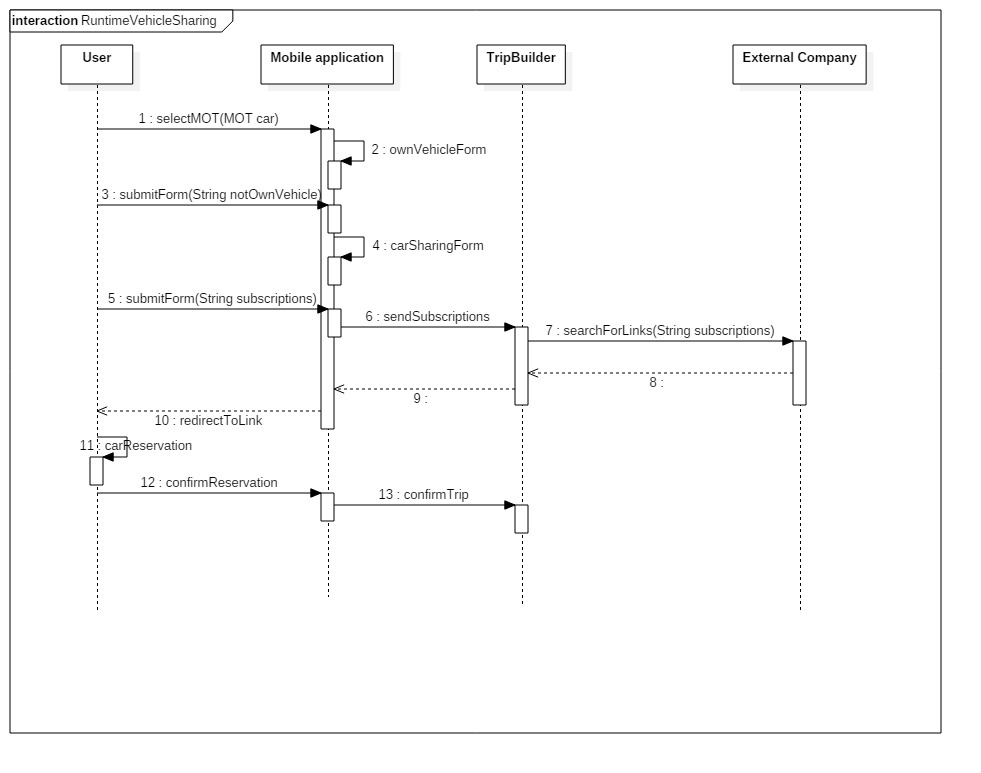
\includegraphics[scale=0.3,]{RuntimeVehicleSharing_191117_1}
	\end{center}
	\caption{Runtime sequence diagram of shared-vehicle reservation}
\end{figure}
\begin{figure}[!h]
	\centering
	\begin{center}
		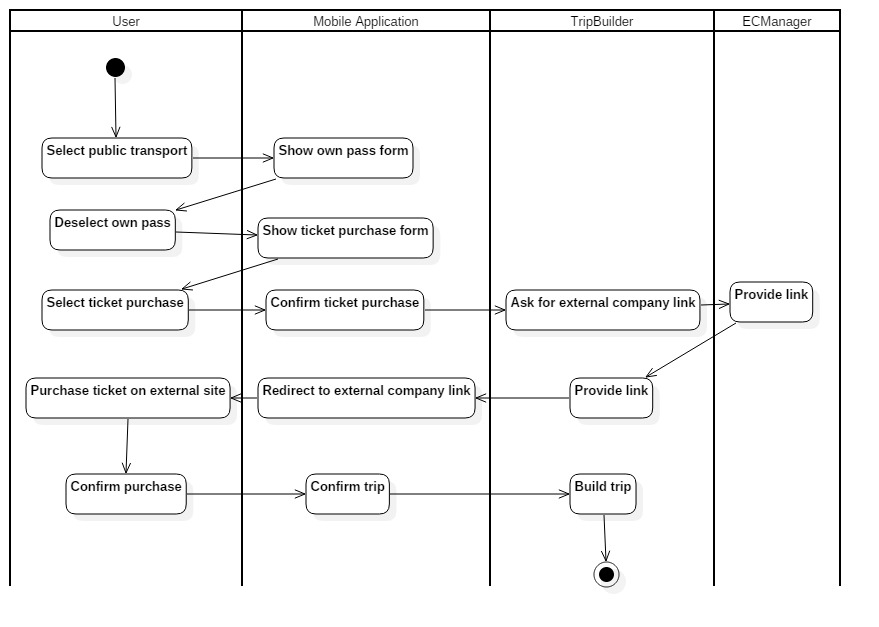
\includegraphics[scale=0.3]{TicketPurchaseActivity_241117_1}
	\end{center}
	\caption{Runtime activity diagram of ticket purchase}
\end{figure}

The top sequence diagram describes the runtime interaction between components during the reservation of a vehicle of a sharing service. A vehicle can be a car, a bike, a 
motorcycle or anything provided by external companies interacting with the system. It refers to use cases 13 and 14 of section 3.2.2 of the RASD.\\
We are in the situation of a meeting creation and the user is selecting the chosen travel means: one of these is a vehicle and the user has not a personal one.
The reservation of a vehicle is perfomed on the external company's website or application; the user is asked for the list of companies for which he or she has a subscription.
Once the reservation is complete, the user confirms the creation of the trip.
A very similar interaction is the purchase of a ticket for a public mean of transport (use case 7 of section 3.2.2 of the RASD), shown in the bottom activity diagram: the user is selecting the travel means during the creation of a meeting and
one of these is a public mean of transport. The user has no personal pass for such transport company. The user is redirected to the company's link, where the purchase
is performed.

\subsection{Component Interfaces}
\subsection{Selected architectural styles and patterns}
Here we describe some of the possible design patterns for the implementation of the system. All the name of classes and inetrfaces refer to the latest version of the class diagram.
\begin{itemize}
	\item Adapter: this pattern has been used to adapt the UserDevice interface to the different operating systems of the users.
	\item Builder
	\item Factory
	\item MVC: this pattern has been overall used to keep separated logic, information and the way they are presented to the user.
	\item Observer: this pattern has been used to manage the notification of problems that may affect travel means, such as strikes or bad weather conditions. The interested classes (MeanOfTransport, Navigator and Trip) are notified when a Notification related to one of such problems changes its status.
	\item Singleton: this pattern has been used for classes that need to be instanciated only a single time; in particular, they are the classes NotificationManager, SystemShared, WindowsPhone, AndroidDevice and iOSDevice
\end{itemize}

\subsection{Other design decisions}

\newpage
\section{Algorithm design}

\newpage
\section{User interface design}

\begin{figure}
\begin{minipage}[!h]{0.45\linewidth}
	\centering
	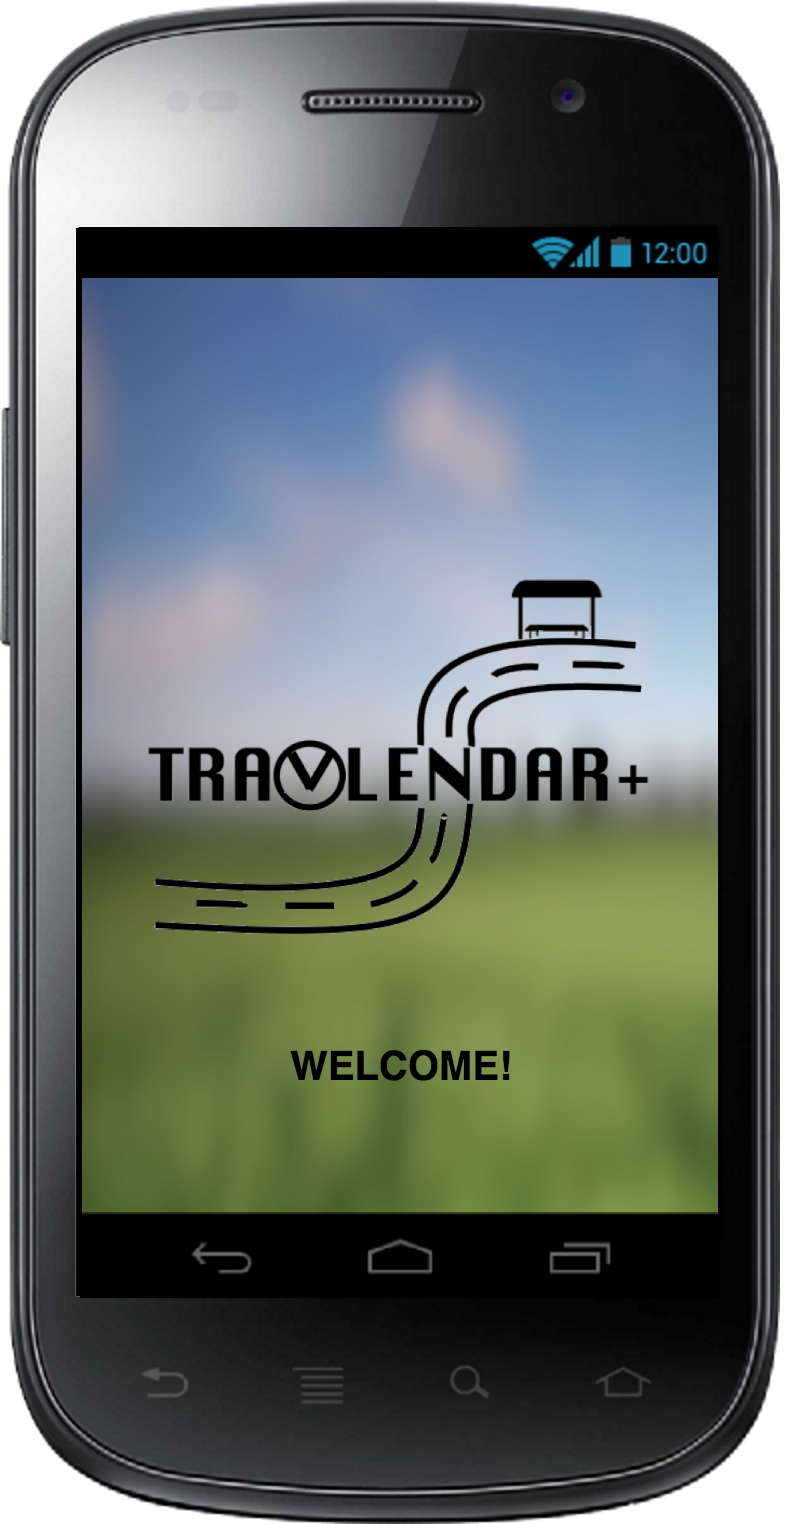
\includegraphics[scale=0.15]{startPage}
	\captionof{figure}{Start page}
\end{minipage}
\hspace{0.5cm}
\begin{minipage}[!h]{0.45\linewidth}
	\centering
	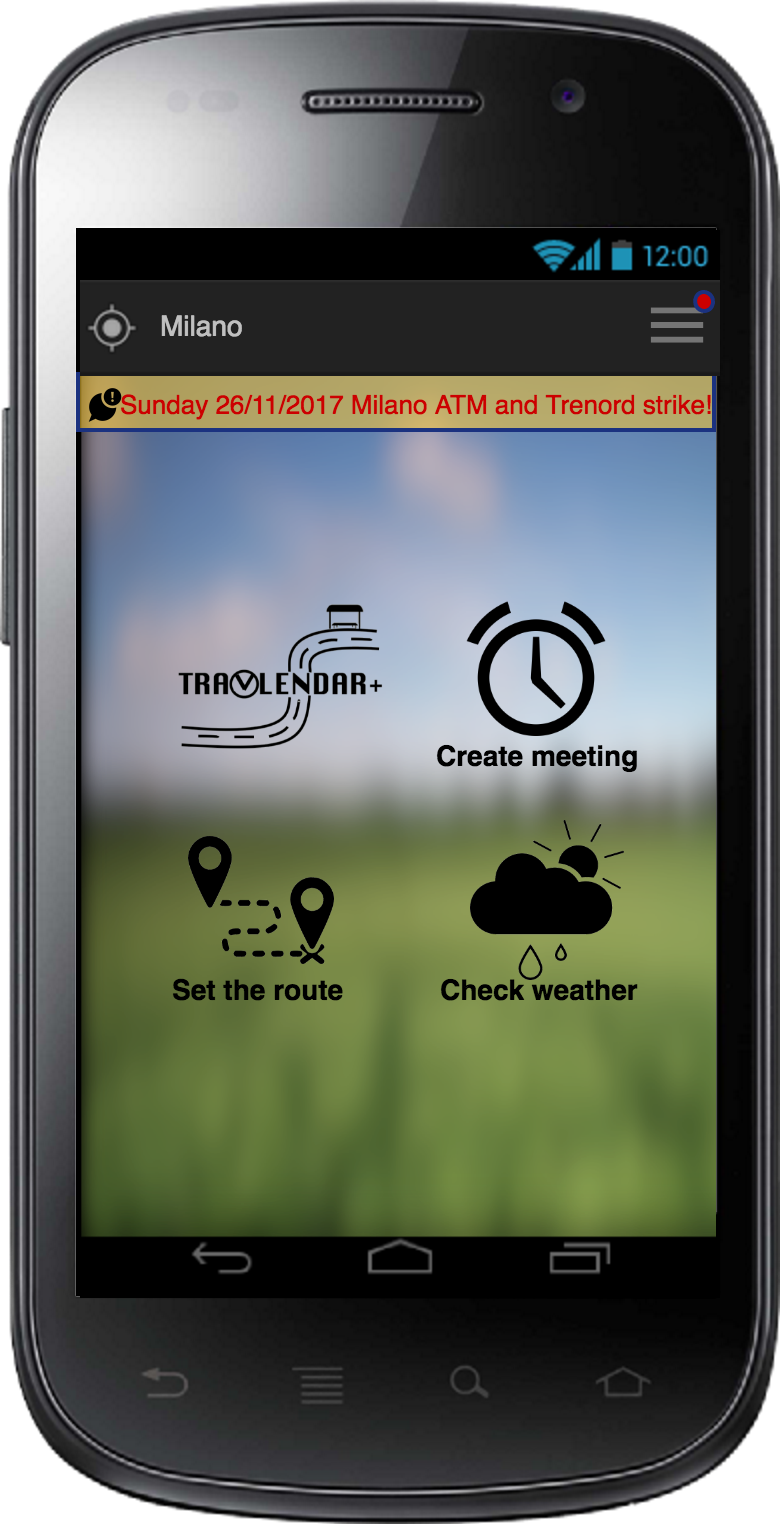
\includegraphics[scale = 0.15]{mainPage.png}
	\captionof{figure}{Main page}
\end{minipage}

\vspace{3.5 cm}

\begin{minipage}[!h]{0.45\linewidth}
	\centering
	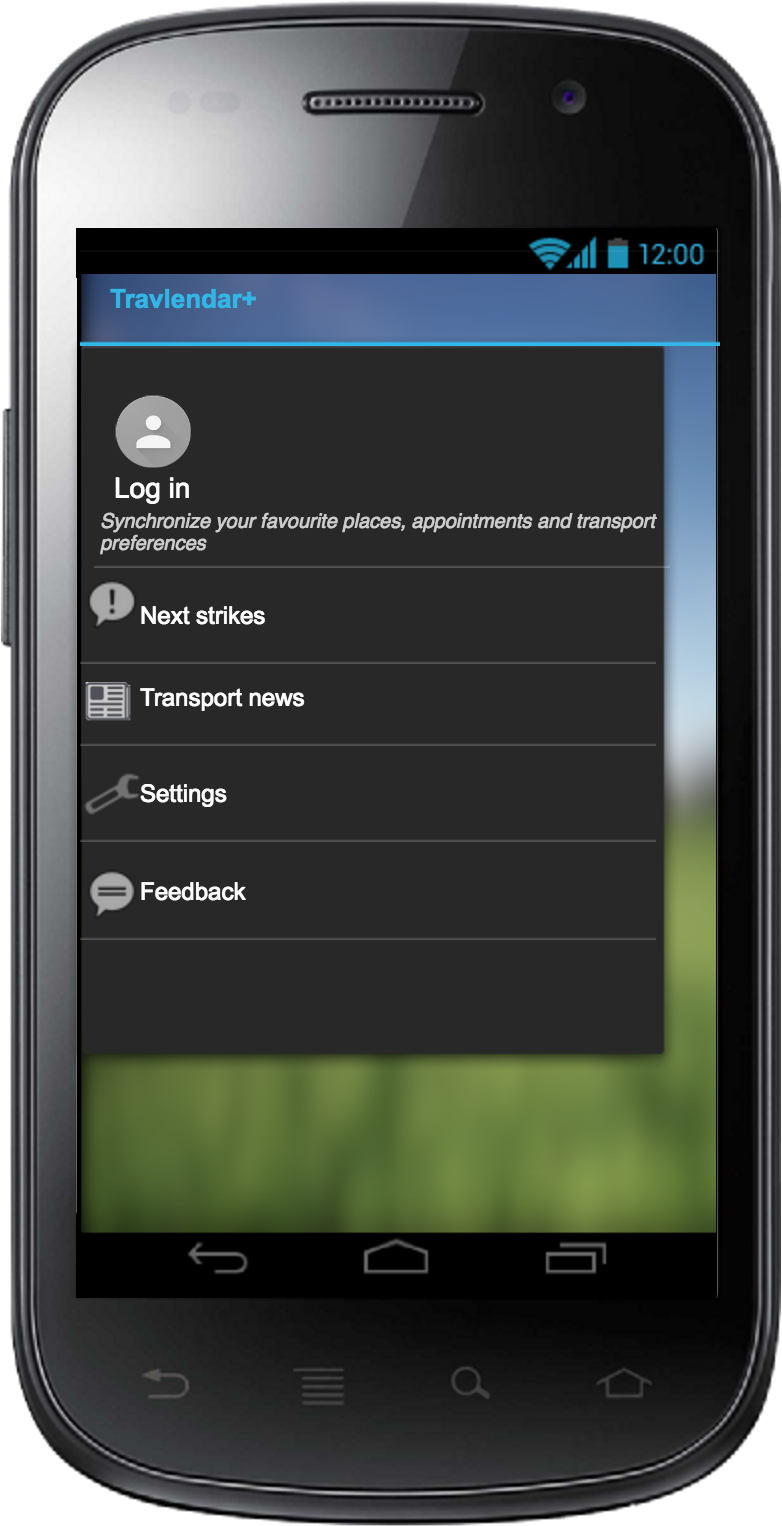
\includegraphics[scale = 0.15]{Menu.png}
	\captionof{figure}{Visitor menu}
\end{minipage}
\hspace{0.5cm}
\begin{minipage}[!h]{0.45\linewidth}
	\centering
	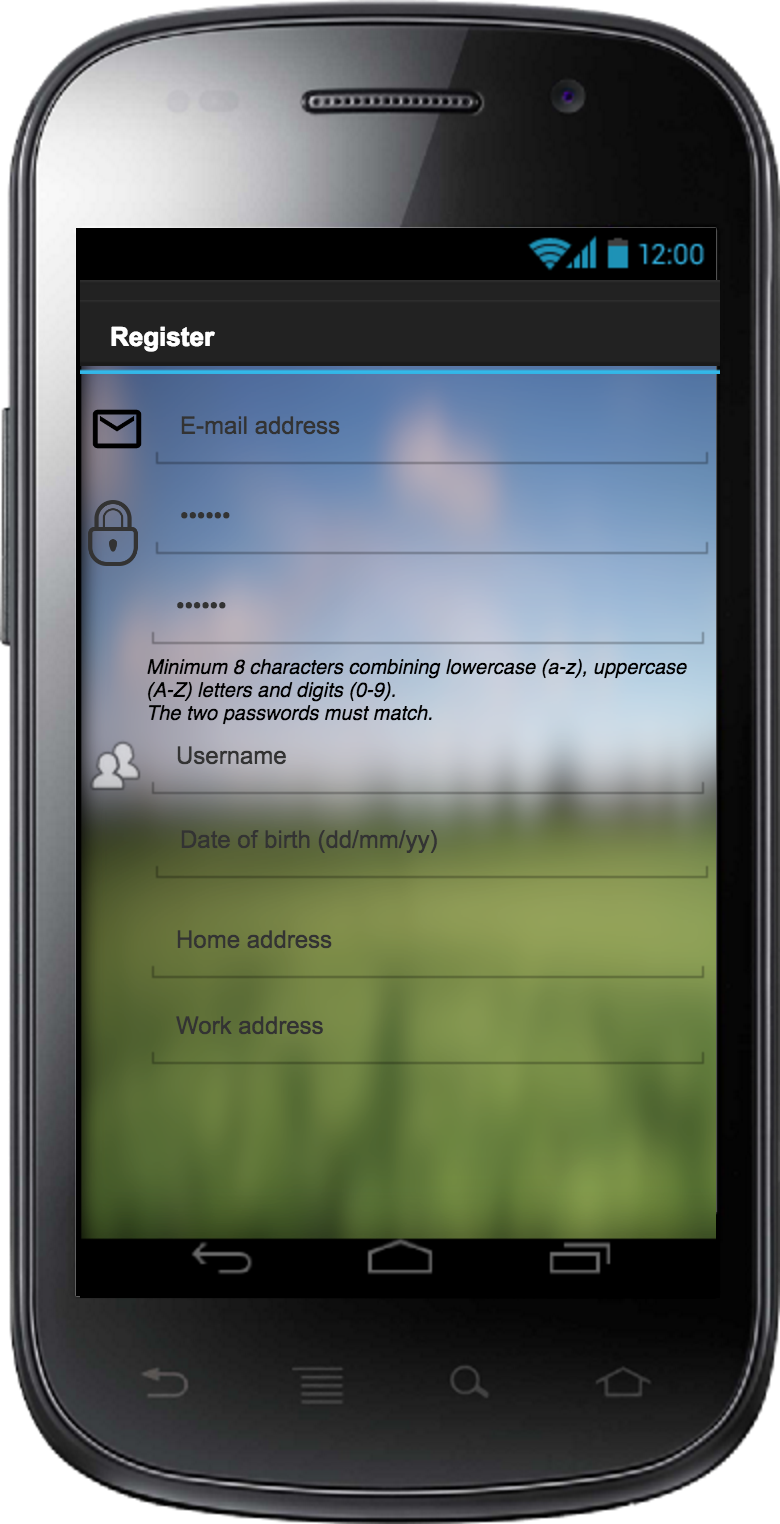
\includegraphics[scale = 0.15]{Registration.png}
	\captionof{figure}{Registration}
\end{minipage}
\end{figure}

\newpage
\begin{figure}
	\begin{minipage}[!h]{0.45\linewidth}
		\centering
		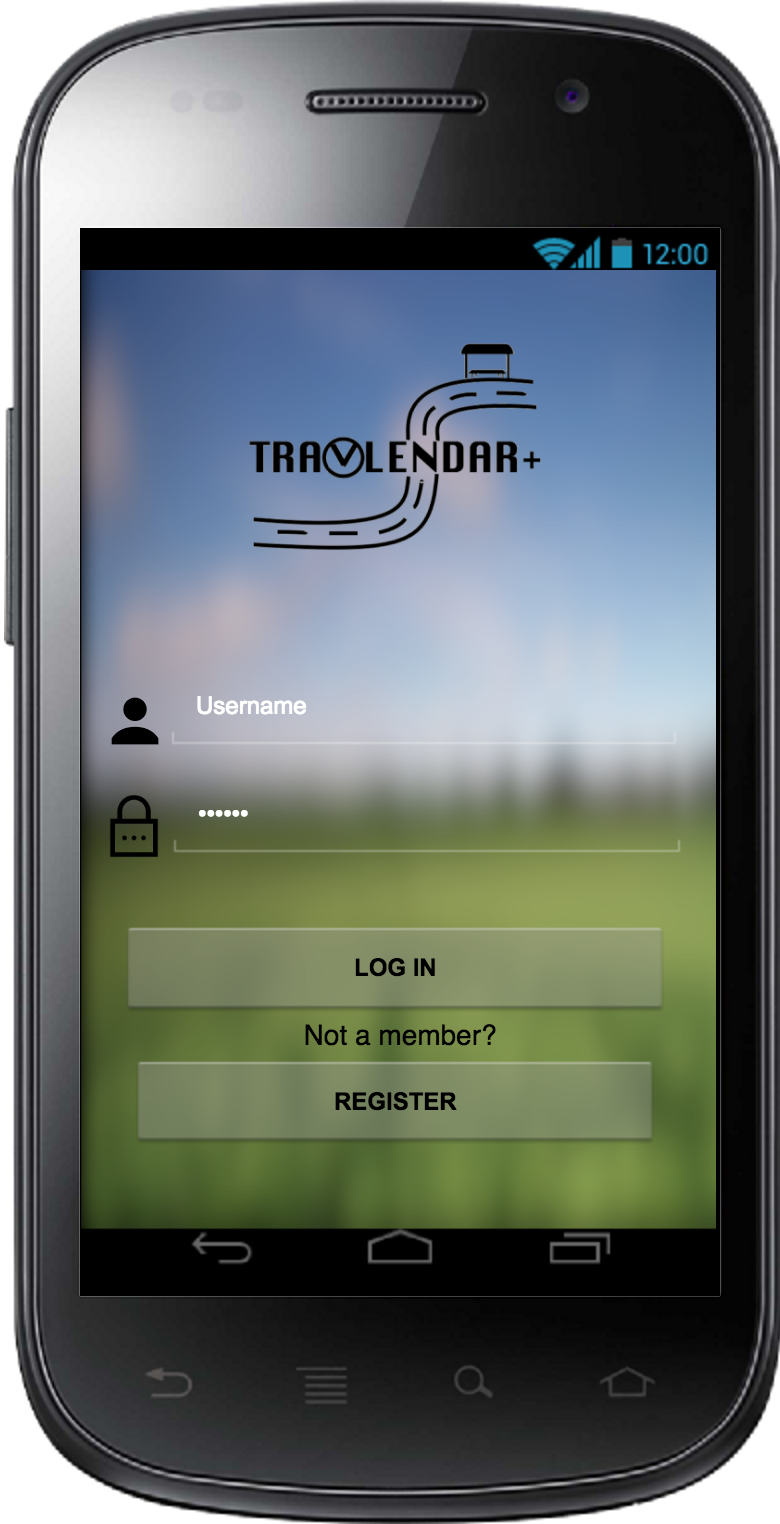
\includegraphics[scale=0.15]{access}
		\captionof{figure}{Login}
	\end{minipage}
	\hspace{0.5cm}
	\begin{minipage}[!h]{0.45\linewidth}
		\centering
		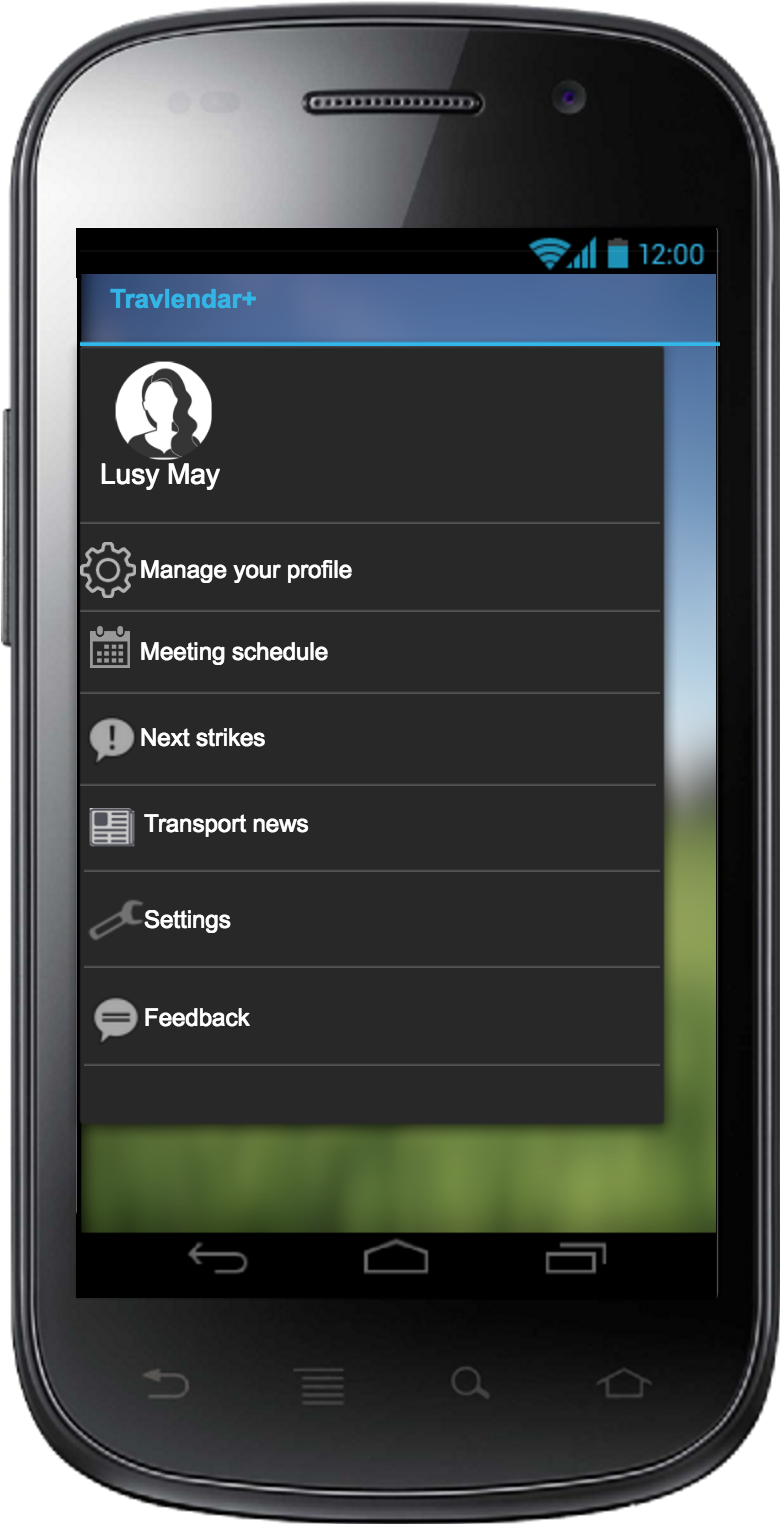
\includegraphics[scale = 0.15]{clientMenu.png}
		\captionof{figure}{Client menu}
	\end{minipage}
	
	\vspace{3.5 cm}
	
	\begin{minipage}[!h]{0.45\linewidth}
		\centering
		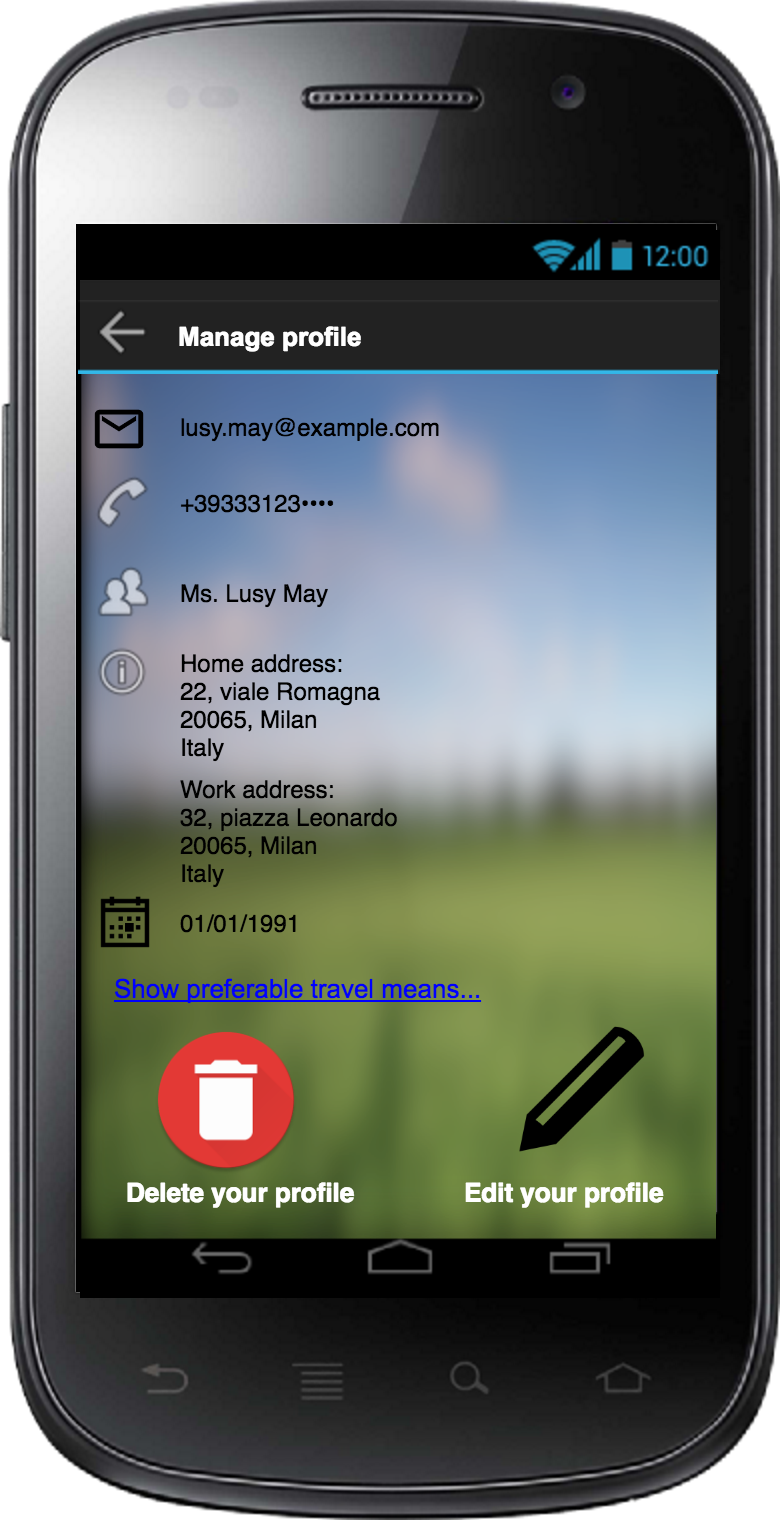
\includegraphics[scale = 0.15]{manageProfile.png}
		\captionof{figure}{Manage profile}
	\end{minipage}
	\hspace{0.5cm}
	\begin{minipage}[!h]{0.45\linewidth}
		\centering
		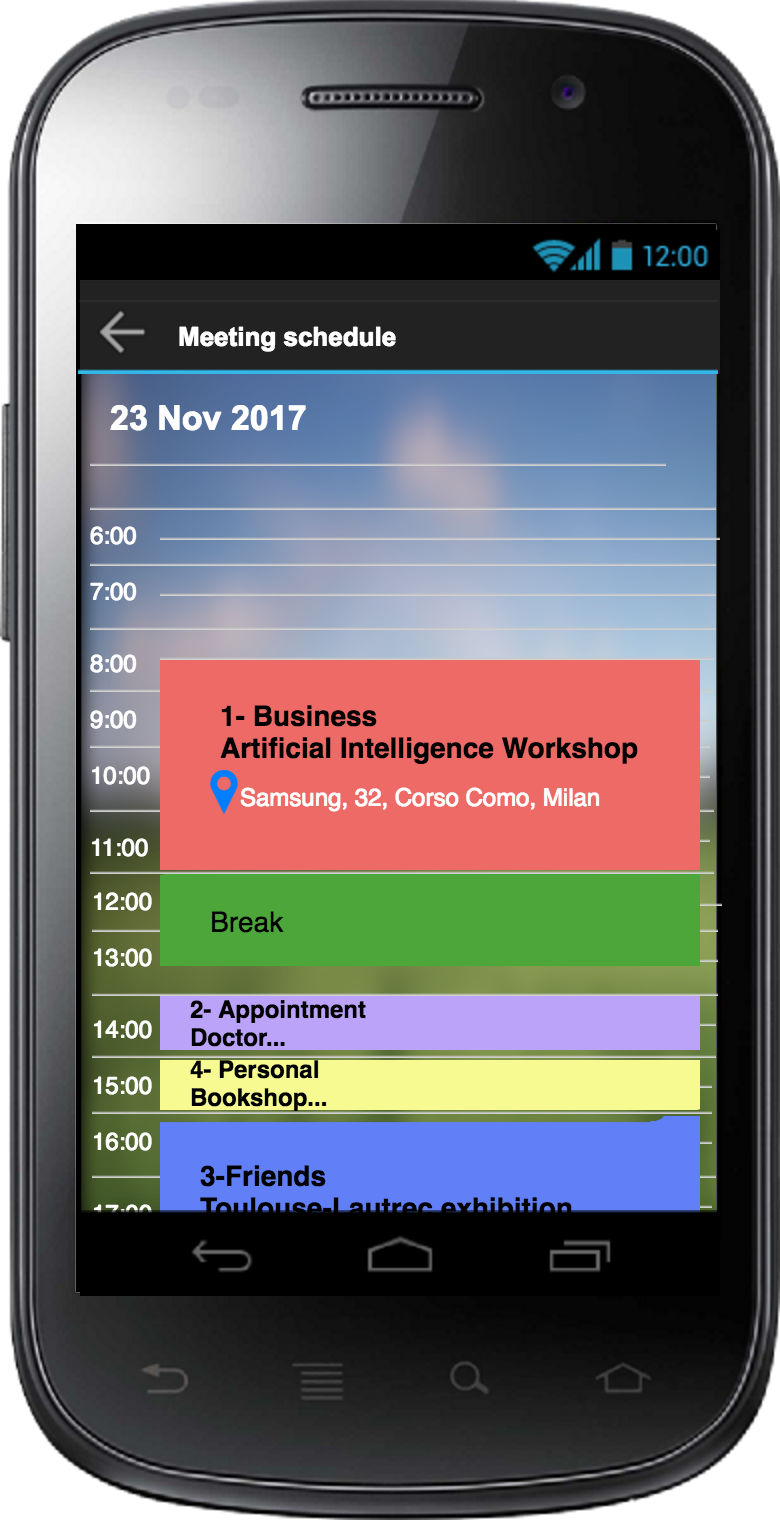
\includegraphics[scale = 0.15]{meetingSchedule.png}
		\captionof{figure}{Schedule of meetings}
	\end{minipage}
\end{figure}

\newpage
\begin{figure}
	\begin{minipage}[!h]{0.45\linewidth}
		\centering
		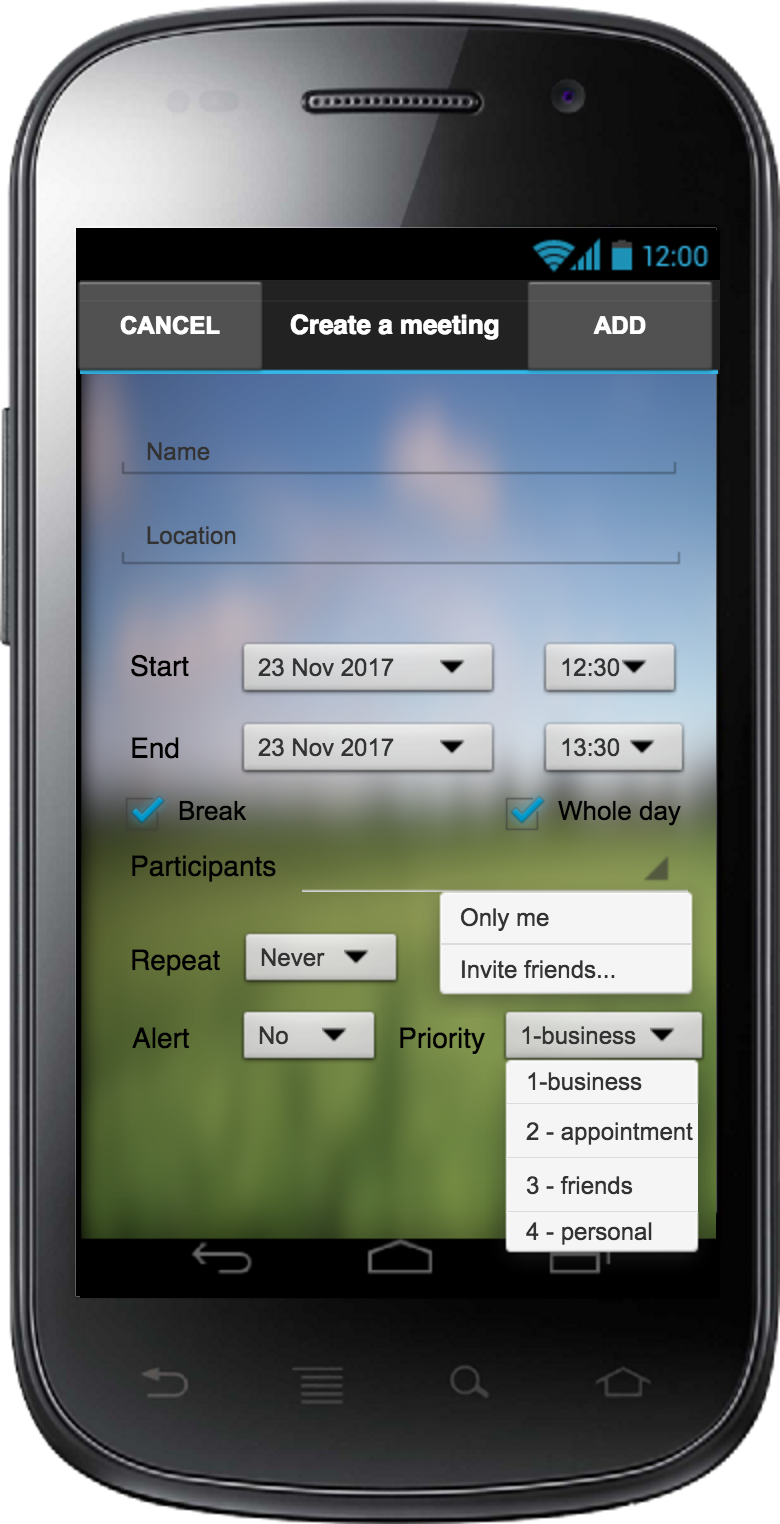
\includegraphics[scale=0.15]{createMeeting}
		\captionof{figure}{Meeting creation}
	\end{minipage}
	\hspace{0.5cm}
	\begin{minipage}[!h]{0.45\linewidth}
		\centering
		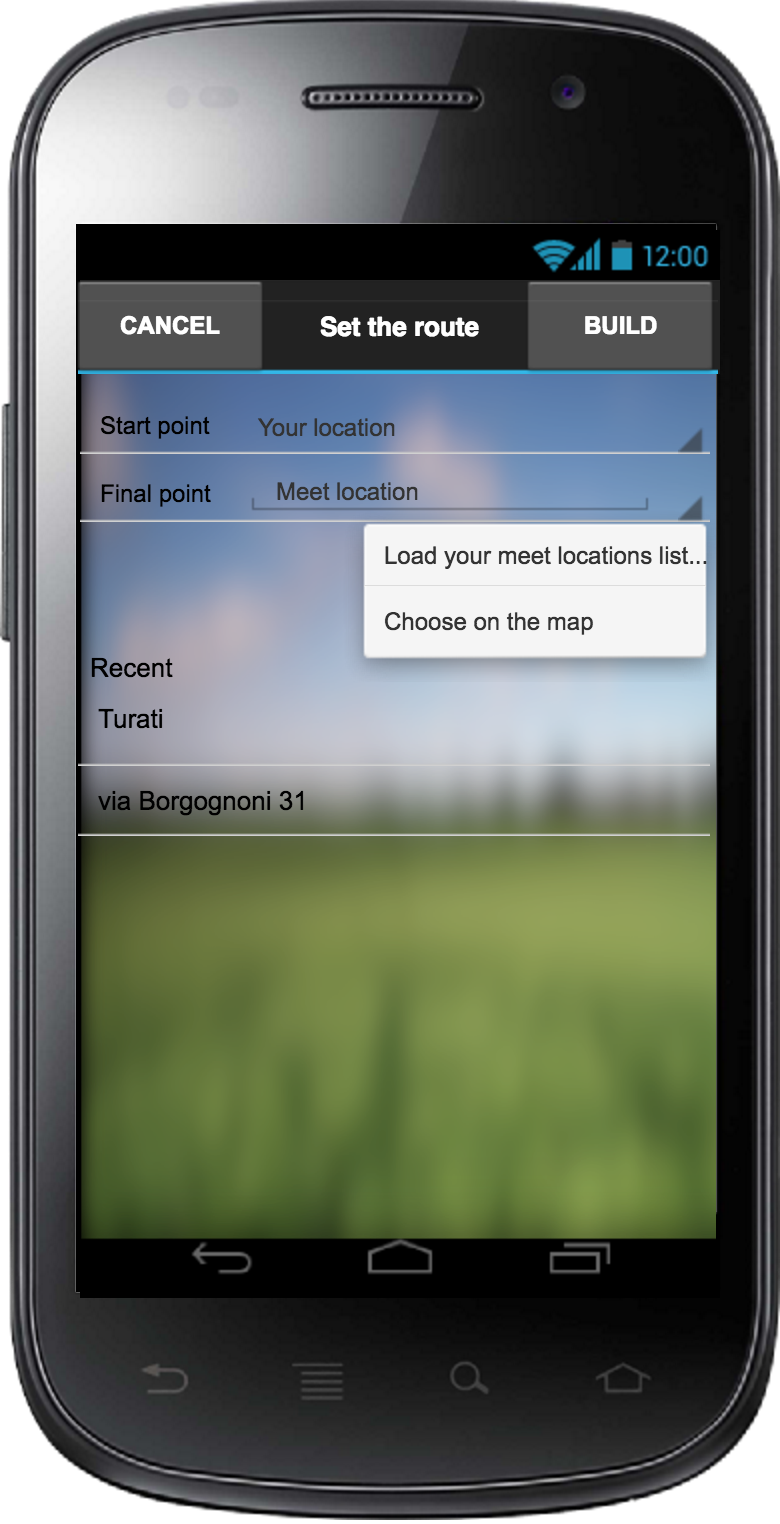
\includegraphics[scale = 0.15]{setRoute.png}
		\captionof{figure}{Set route}
	\end{minipage}
	
	\vspace{3.5 cm}
	
	\begin{minipage}[!h]{0.45\linewidth}
		\centering
		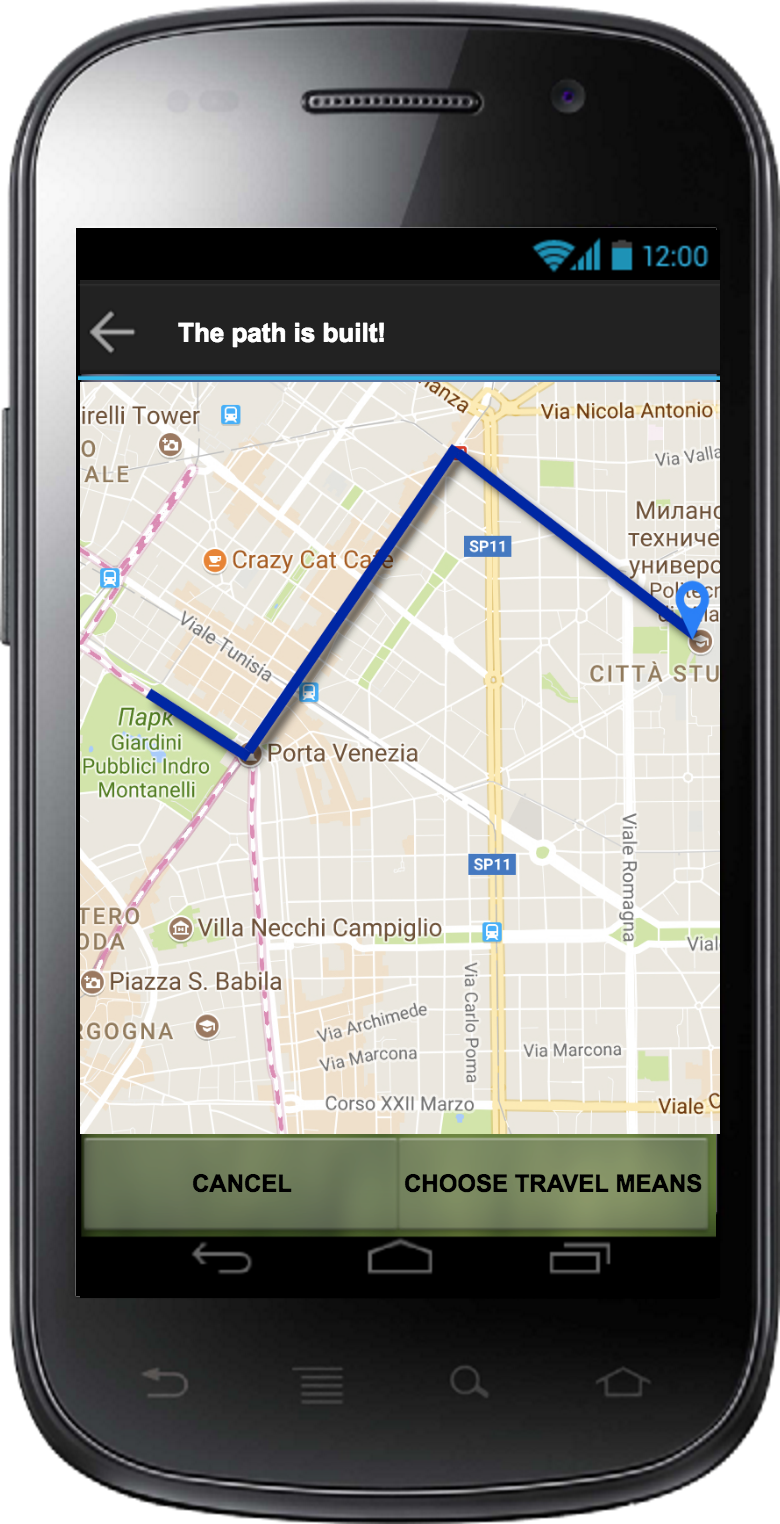
\includegraphics[scale = 0.15]{buildPath.png}
		\captionof{figure}{Path building}
	\end{minipage}
	\hspace{0.5cm}
	\begin{minipage}[!h]{0.45\linewidth}
		\centering
		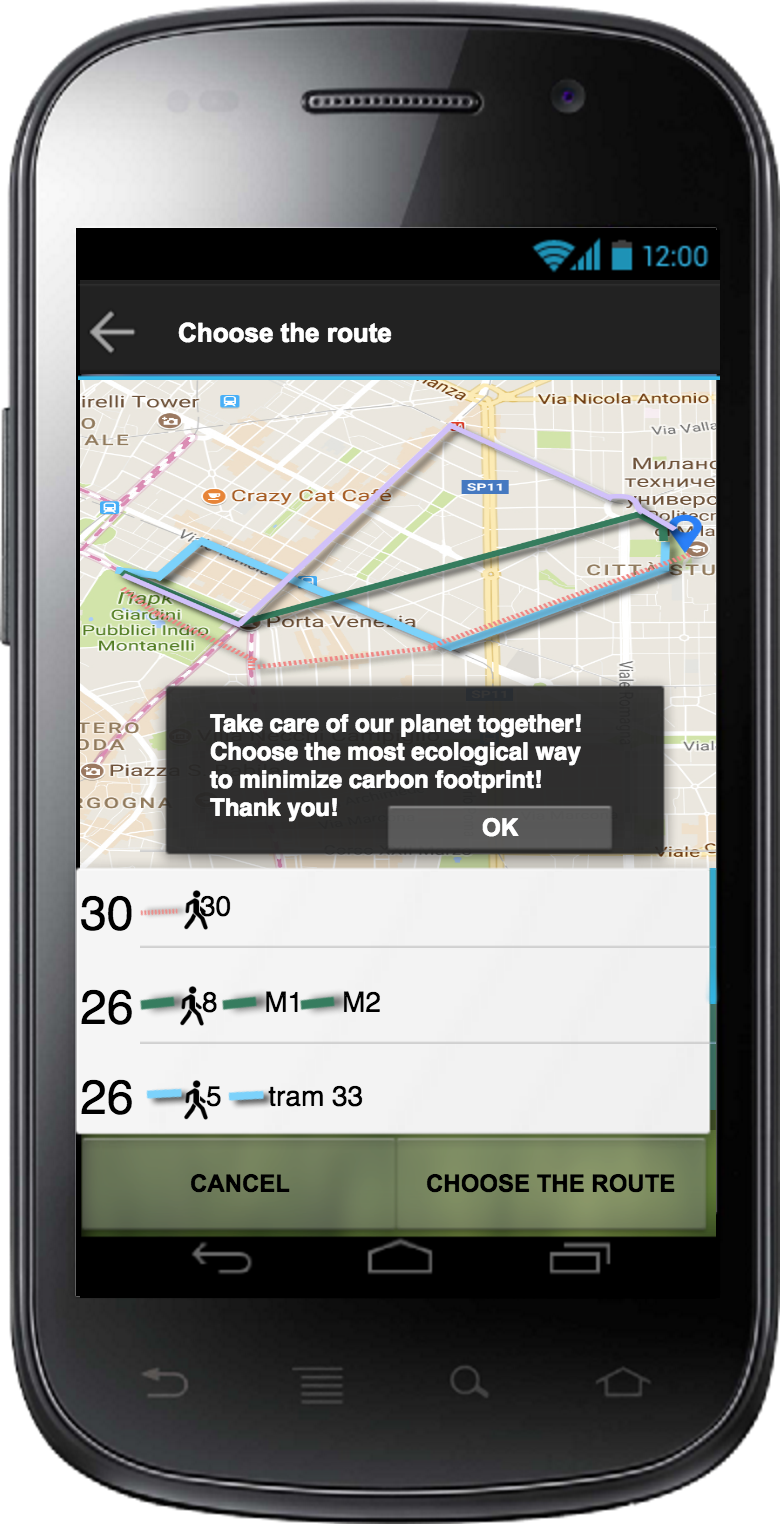
\includegraphics[scale = 0.15]{buildRoute.png}
		\captionof{figure}{Route building}
	\end{minipage}
\end{figure}

\newpage
\begin{figure}
	\begin{minipage}[!h]{0.45\linewidth}
		\centering
		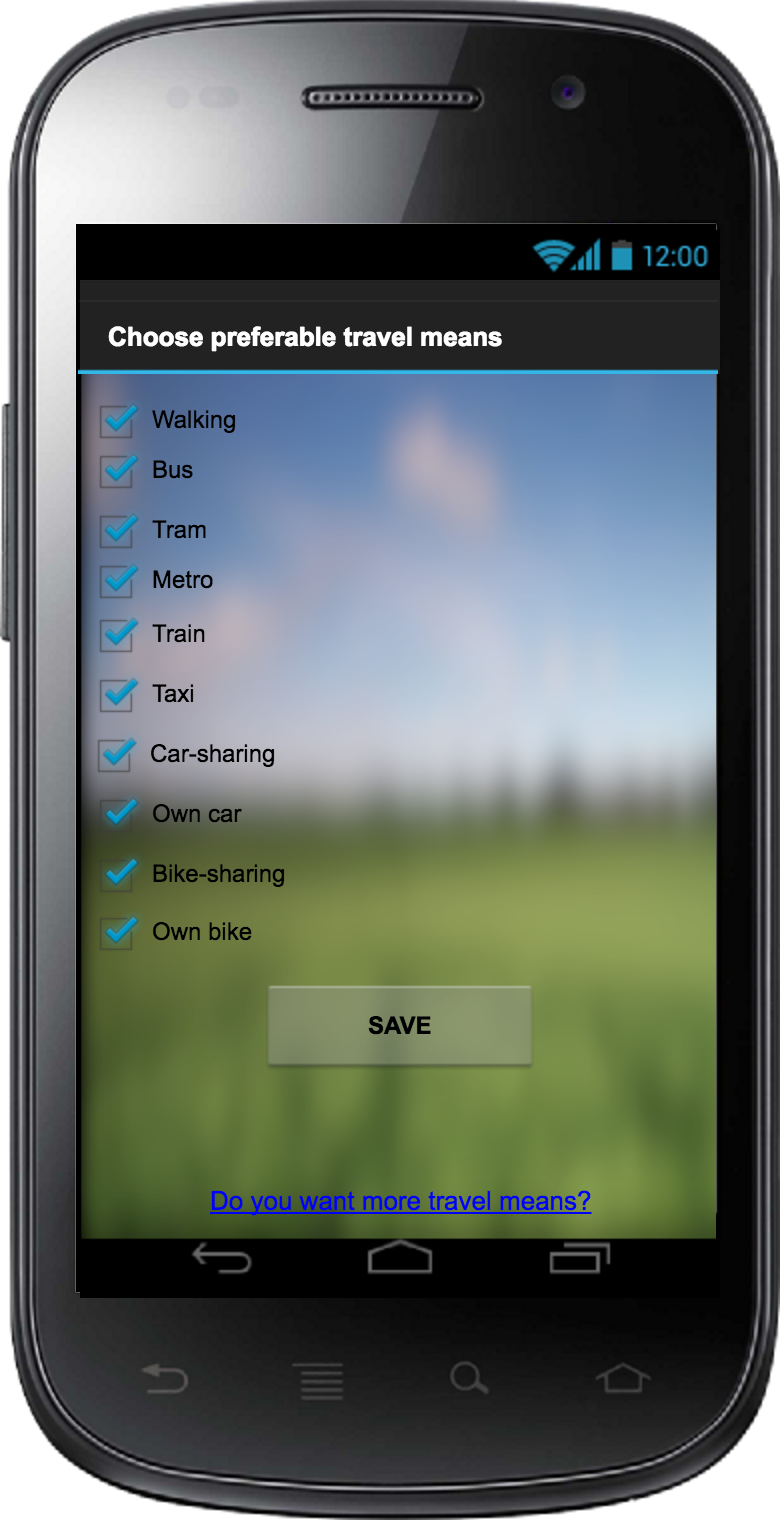
\includegraphics[scale=0.15]{choosePrefTransport}
		\captionof{figure}{Choice of preferable means}
	\end{minipage}
	\hspace{0.5cm}
	\begin{minipage}[!h]{0.45\linewidth}
		\centering
		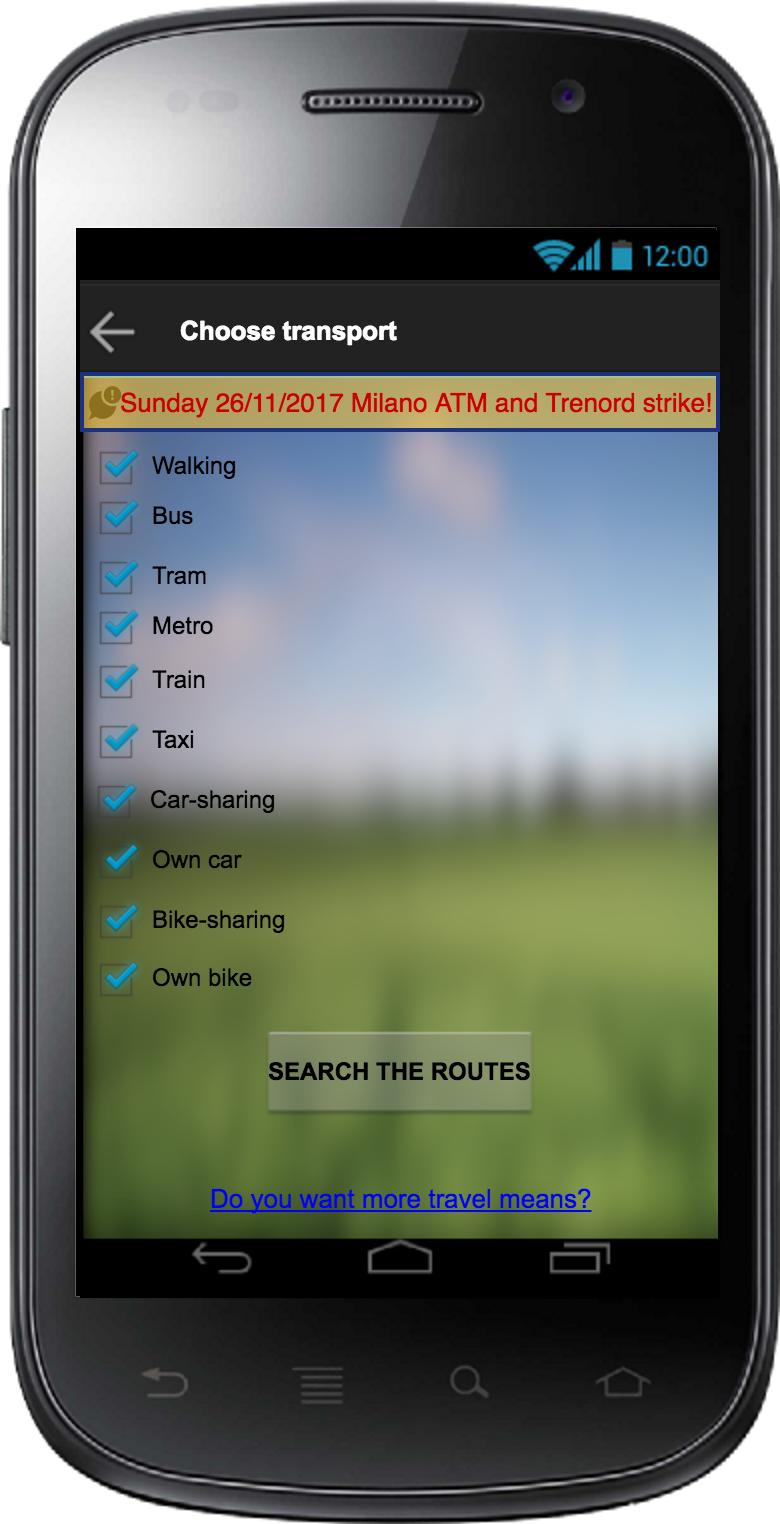
\includegraphics[scale = 0.15]{chooseTransport.png}
		\captionof{figure}{Choice of mean of transport}
	\end{minipage}
	
	\vspace{3.5 cm}
	
	\begin{minipage}[!h]{0.45\linewidth}
		\centering
		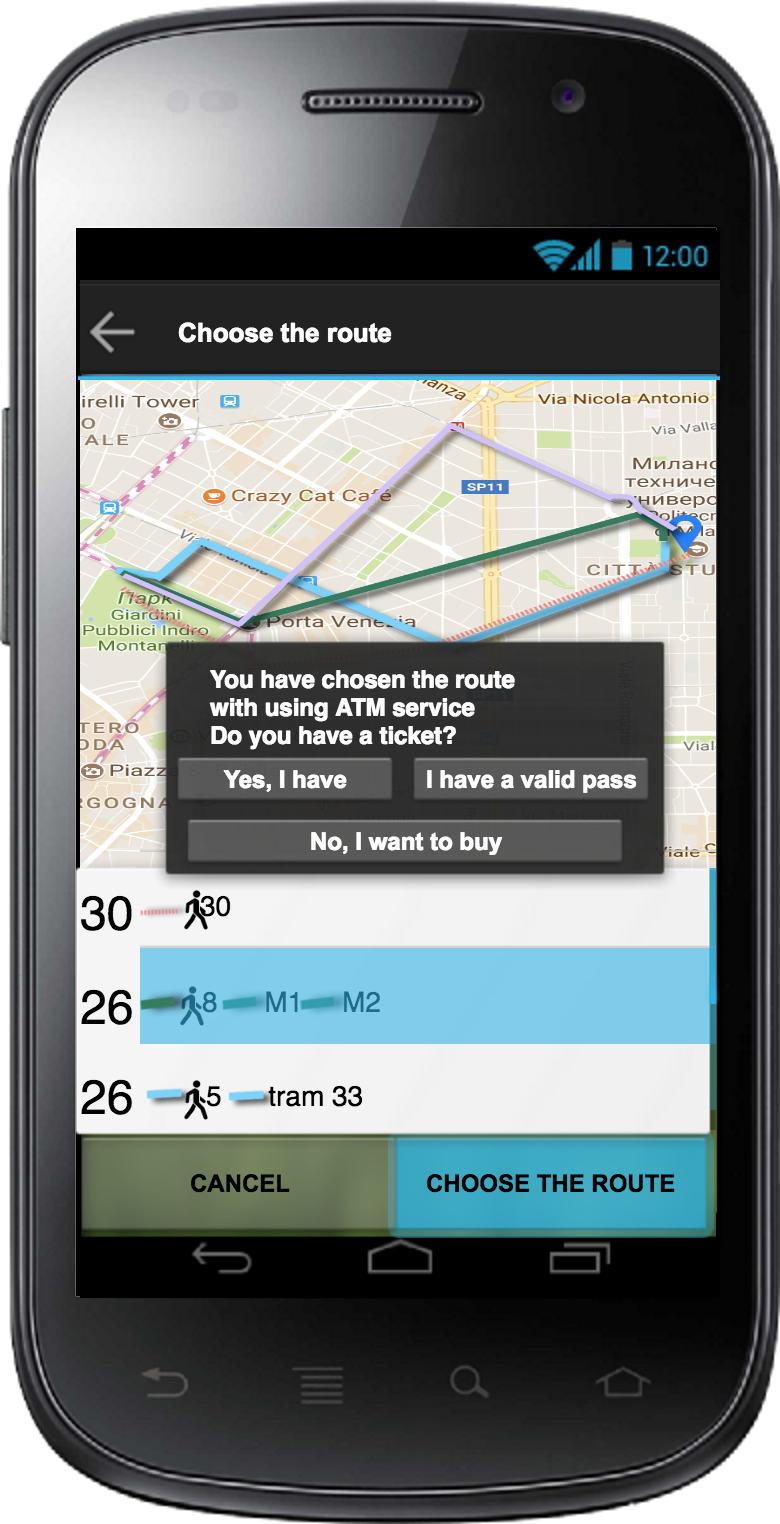
\includegraphics[scale = 0.15]{buyTicket.png}
		\captionof{figure}{Purchase of ticket}
	\end{minipage}
	\hspace{0.5cm}
	\begin{minipage}[!h]{0.45\linewidth}
		\centering
		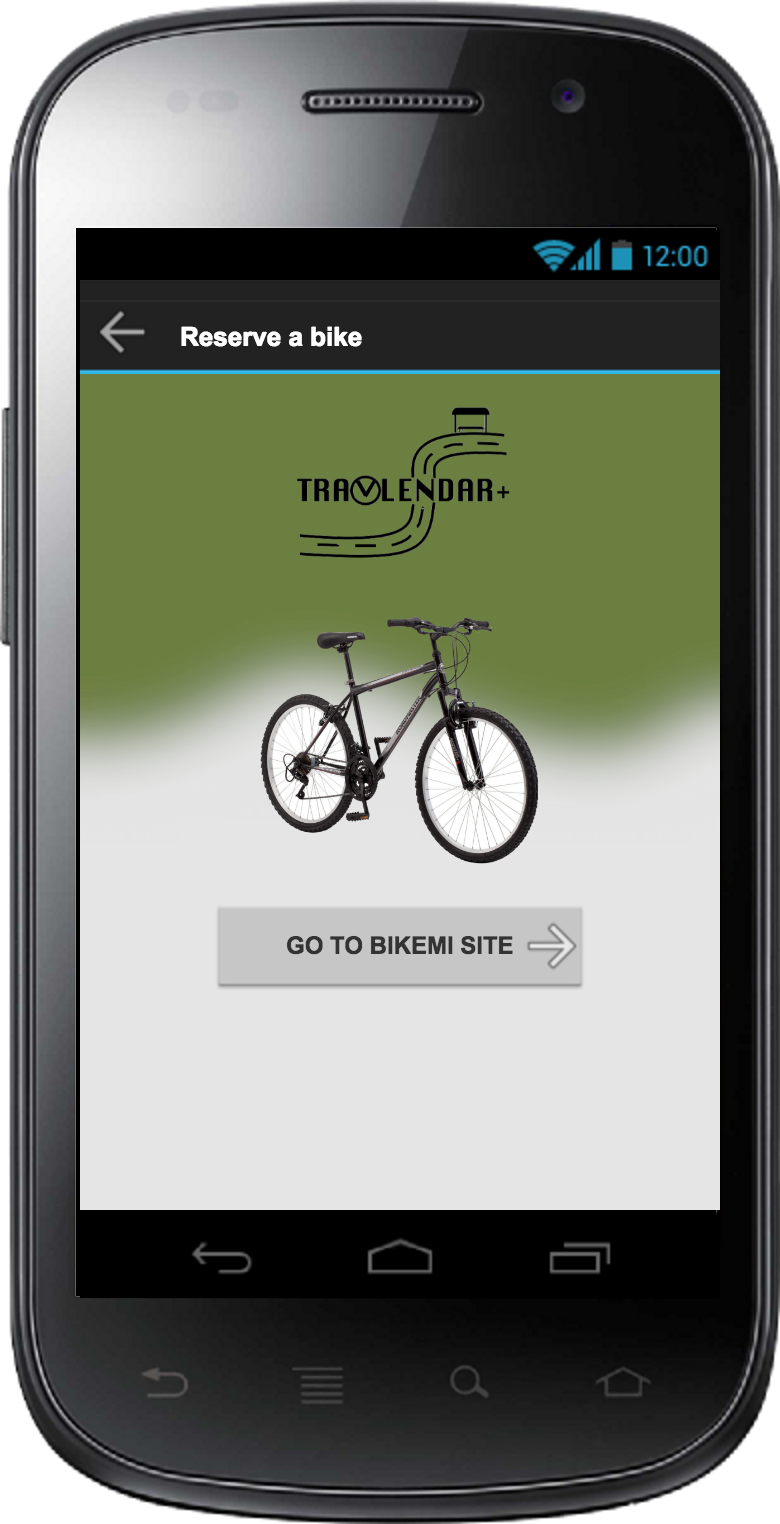
\includegraphics[scale = 0.15]{reserveBike.png}
		\captionof{figure}{Reservation of bike}
	\end{minipage}
\end{figure}

\newpage
\begin{figure}
	\begin{minipage}[!h]{0.45\linewidth}
		\centering
		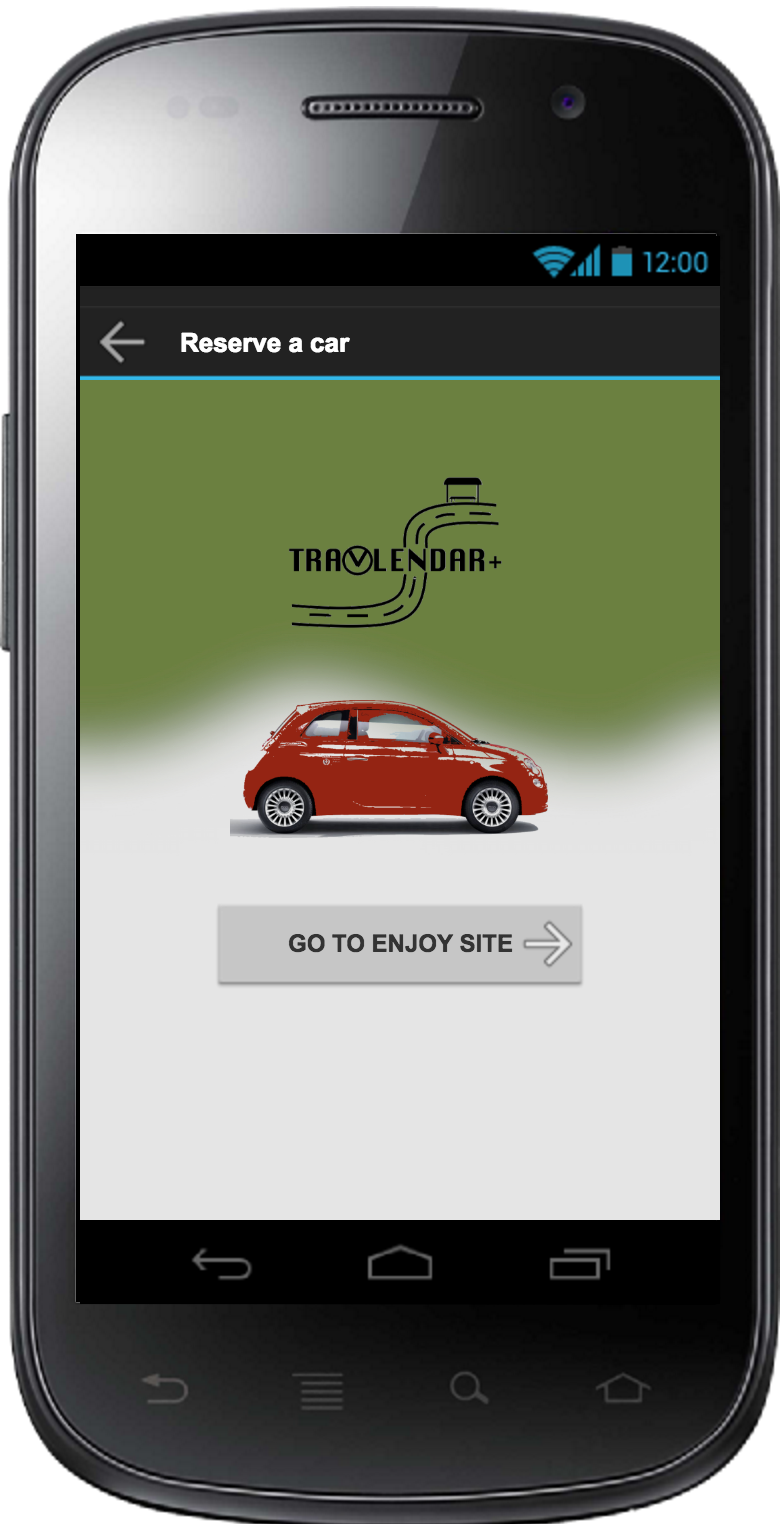
\includegraphics[scale=0.15]{reserveCar}
		\captionof{figure}{Reservation of car}
	\end{minipage}
	\hspace{0.5cm}
	\begin{minipage}[!h]{0.45\linewidth}
		\centering
		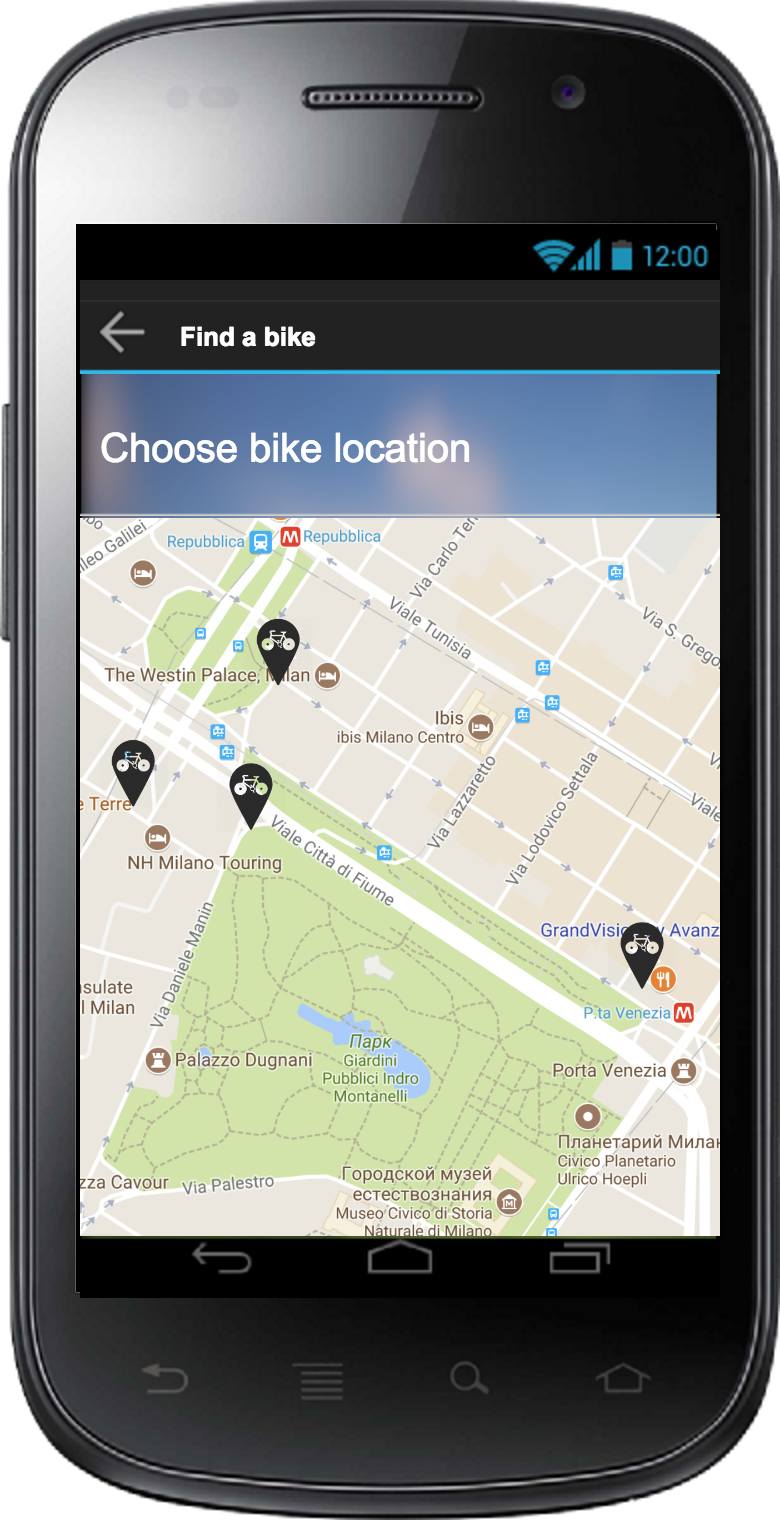
\includegraphics[scale = 0.15]{findBike.png}
		\captionof{figure}{Position of bikes of bike-sharing service}
	\end{minipage}
	
	\vspace{3.5 cm}
	
	\begin{minipage}[!h]{0.45\linewidth}
		\centering
		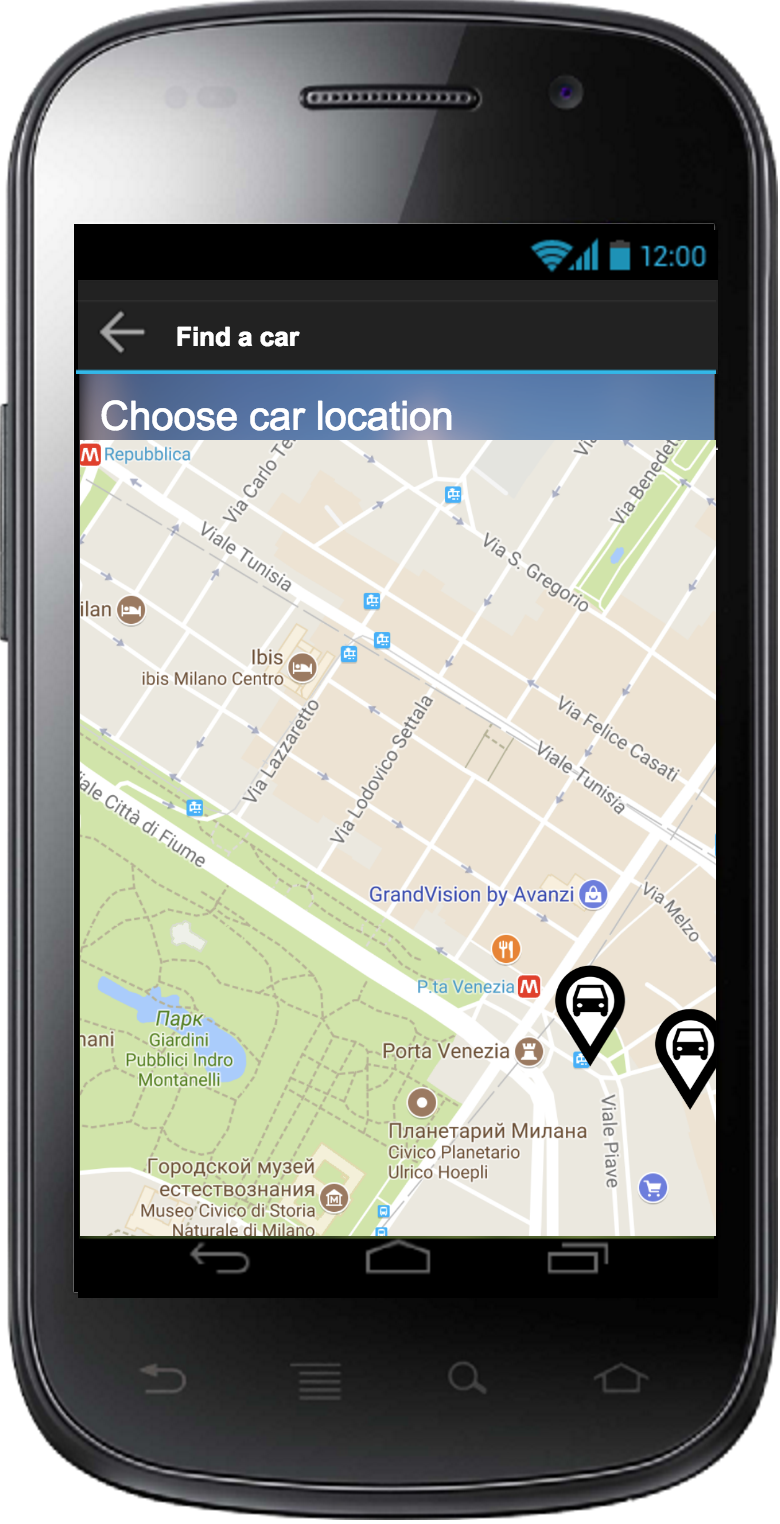
\includegraphics[scale = 0.15]{findCar.png}
		\captionof{figure}{Position of cars of car-sharing service}
	\end{minipage}
\end{figure}

\newpage
\section{Requirements traceability}
In this section we identify which components or functionalities are responsible for the goals and requirements stated in the RASD.

\begin{itemize}
	
	\item (G01): The software should allow the user to register.
	\begin{itemize}
		\item (RE01): The system must allow users to sign in: Mobile application, LoginController, Model, Database
		\item (RE02): The system must allow the client to log in: Mobile Application, LoginController, Model, Database
		\item (RE03): The system must allow the client to log out: Mobile Application, LoginController
		\item (RE04): The system must allow the client to delete his account: Mobile Application, LoginController, Model, Database
		\item (RE05): The system must provide a high level of security for client's data: LoginController, Model, Database
	\end{itemize}
	\item (G02): The system allows User to set his/her route inside a city or a region.
	\begin{itemize}
		\item (RE08): The software must allow the user to choose a route: Mobile Application, MeetingController, TripController, NavigatorController, Model
		\item (RE09): The software must allow the user to define time constraint to a specific selected route: Mobile Application, MeetingController, Model
	\end{itemize}
	\item (G03): The system allows a User to choose a kind of transport among pre-defined travel means according to his/her preferences
	\begin{itemize}
		\item (RE10): For each path the software must provide all the available means of transport that can be used, according to the software interfaces: Mobile Application, TripController, ExternalCompanyController
		\item (RE11): The software must allow the user to select vehicles that he/she wants to use for the route: Mobile Application, MeetingController, Model
		\item (RE15): If a route is not possible because the selected travel mean is not allowed to pass a specific place, the application must deny that option and notify the user: Mobile Application, PathRestrictionController
	\end{itemize}
	\item (G04): The system allows a User to reserve a range of time for breaks.
	\begin{itemize}
		\item (RE12): The software must require the estimated time for a break: Mobile Application, BreakController 
		\item (RE16): If a route is not possible because breaks requires too much time, the application must deny that option and notify the user: Mobile Application, BreakController
		\item (RE20): If a break runs out the selected time the application must notify the user: Mobile Application, BreakController
	\end{itemize}
	\item (G05): The system must communicate to the user that a path (selected by this one) is not reachable or it's out of time.
	\begin{itemize}
		\item (RE14): If a route is not possible because the required time to reach the destination is not enough, the application must deny that option and notify the user: Mobile Application, MeetingController
	\end{itemize}
	\item (G06): The system must provide all the possible path that can be taken by a user, according to his/her needs.
	\begin{itemize}
		\item (RE17): The software must provide a User all the available solutions, according to his/her selected preferences, to get from one place to another: Mobile Application, TripController
	\end{itemize}
	\item (G07): The system must provide firstly the most optimized and suitable solution, according to the user preferences.
	\begin{itemize}
		\item (RE19): The application should provide, as first option, the optimal solution according to the users's preferences about minimizing carbon footprint: Mobile Application,  MeetingController, TripController, UserPreferencesController
	\end{itemize}
	\item (G08): The system must provide information about problems/strikes for all the travel means  included in the software.
	\begin{itemize}
		\item (RE18): The software must inform the user about problems with using some transport (strikes , road damages, rain and so on) for which the usability is not guaranteed: Mobile Application, ExternalCompanyController, NotificationManagerController
		\item (RE21): The application should avoid to make the user pass through dangerous zones of a city or a region: TripBuilder, ECManager
		\item (RE22): If the user has to pass through a dangerous zone, the application must inform him/her: Mobile Application, ExternalCompanyController, NotificationManagerController
	\end{itemize}
	\item (G09): The system must provide a user the information about weather conditions during his/her planned route: Mobile Application, ExternalCompanyController, NotificationManagerController
	\item (G10): The system must provide a way to permit a user to buy a ticket for public transports.
	\begin{itemize}
		\item (RE07): The software must interface with all major public transport companies that provide API: APIManager
	\end{itemize}
	\item (G11): The system must provide the nearest location of a bike provided by a pre-defined bike sharing service provider: TripController, ExternalMeanOfTransportCompanyController
	\item (G12): The system must provide the nearest location of a car provided by a pre-defined car sharing service provider: TripController, ExternalMeanOfTransportCompanyController
	\item (G13): The system must avoid overlaps in user's scheduled travels.
	\begin{itemize}
		\item (RE13): If a route is not possible because of overlaps with other journeys, the application must deny that option and notify the user: MeetingController, Model
	\end{itemize}
	\item (G14): The system must allow the user to create meetings with different priority.
	\begin{itemize}
		\item (RE23):  The software must require the estimated time for a meeting: Mobile Application, MeetingController
		\item (RE24): For each meeting, the system should ask the user to define its priority (1-business, 2-appointment, 3-with friends, 4-personal): Mobile Application, MeetingController
	\end{itemize}
	\item (G15): The system must inform the user about upcoming meetings.
	\begin{itemize}
		\item (RE25): The system should warn about upcoming meetings twenty minutes before: PushGateway
	\end{itemize}
	\item (G16): The system must allow the user to change the part of the path during his/her trip: Mobile Application, MeetingController, TripController
	\item (G17): The system must provide an alternative path in case of problems along the selected one: Mobile Application, TripController, ExternalCompanyManager, ExternalMeanOfTransportCompanyManager
	\item (G18): The software should show a user, if possible, the combination of travel means that minimize the carbon footprint, according to the selected path and the required time: Mobile Application, TripController, MeetingController
	
\end{itemize} 

\newpage
\section{Implementation, integration and test plan}

\subsection{Implementation plan}

\subsubsection{Identifying milestones and taskes}
This section aims to point out some of the main concepts and principles according to which tasks and activities were born afterwards. During the development of the project our implementation team deals with the set of Stakeholders. In this set there are included at least one person to represent all the actors defined in RASD and, in particular, a possible User, Financial partners and Sponsors, possible members of the external partneship companies such as Trenord, ATM, Bike-Sharing and Car-sharing services, a possible ISP's member. As a result it will be possible to implement the system legally and fully integrate it with the external environment.

Another topic to discuss is the importance of cost. Cost monitoring is always necessary and formulation of other strategies really depends on the budget and Sponsors and Partners' investments.

There are some milestones during the liife cycle of the Project:
\begin{itemize}
	\item Implementation phase -- includes concrete implementation (abstract classes and interface development) and testing of the most important parts of the Project software.
	\item Deployment phase -- it is the range of time that is necessary to prepare the Project to be potentially lauched into the market.
	\item Maintenance phase -- includes revisioning the Project and its code, fixing bugs, which has not been distinguished during the testing, and further implementation according to precise scheme and first feedback from Users.
\end{itemize}

So it is crucial to develop the Project and update its releases with new interactive functionalities after Startup period to conform new tendencies and future. The methology of the Project implementation is Agile.

\subsubsection{Schedule}
In this section there is presented the schedule of Travlendar+ Project. It is a high-level general schedule that allows to make clear the main tasks and phases of the Project implementation.

There are represented the main tasks of project implementation:
\begin{itemize}
	\item Prototype implementation
	\item Platform installation and setup
	\item Database implementation
	\item Server subcomponents implementation
	\item Mobile app subcomponents implementation
	\item Prototype testing
	\item Unit testing
	\item Integration testing
	\item System testing
	\item First Internal simulation (Server side analysis)
	\item First Internal simulation (Mobile App side analysis)
	\item Bug fixes
	\item Second Internal simulation (Mobile App side analysis)
	\item Bug fixes, Code inspection
	\item Concrete components integration testing
	\item Documentation and Demonstration
	\item First Internal Demonstration
	\item Second Internal Demonstration
	\item Implementation and Test deliverable (ITD), \item User manual
	\item Acceptance Test deliverable (ATD)
	\item Project presentation for Stakeholders
	
\end{itemize}

\begin{figure}[!h]
	\begin{centering}
		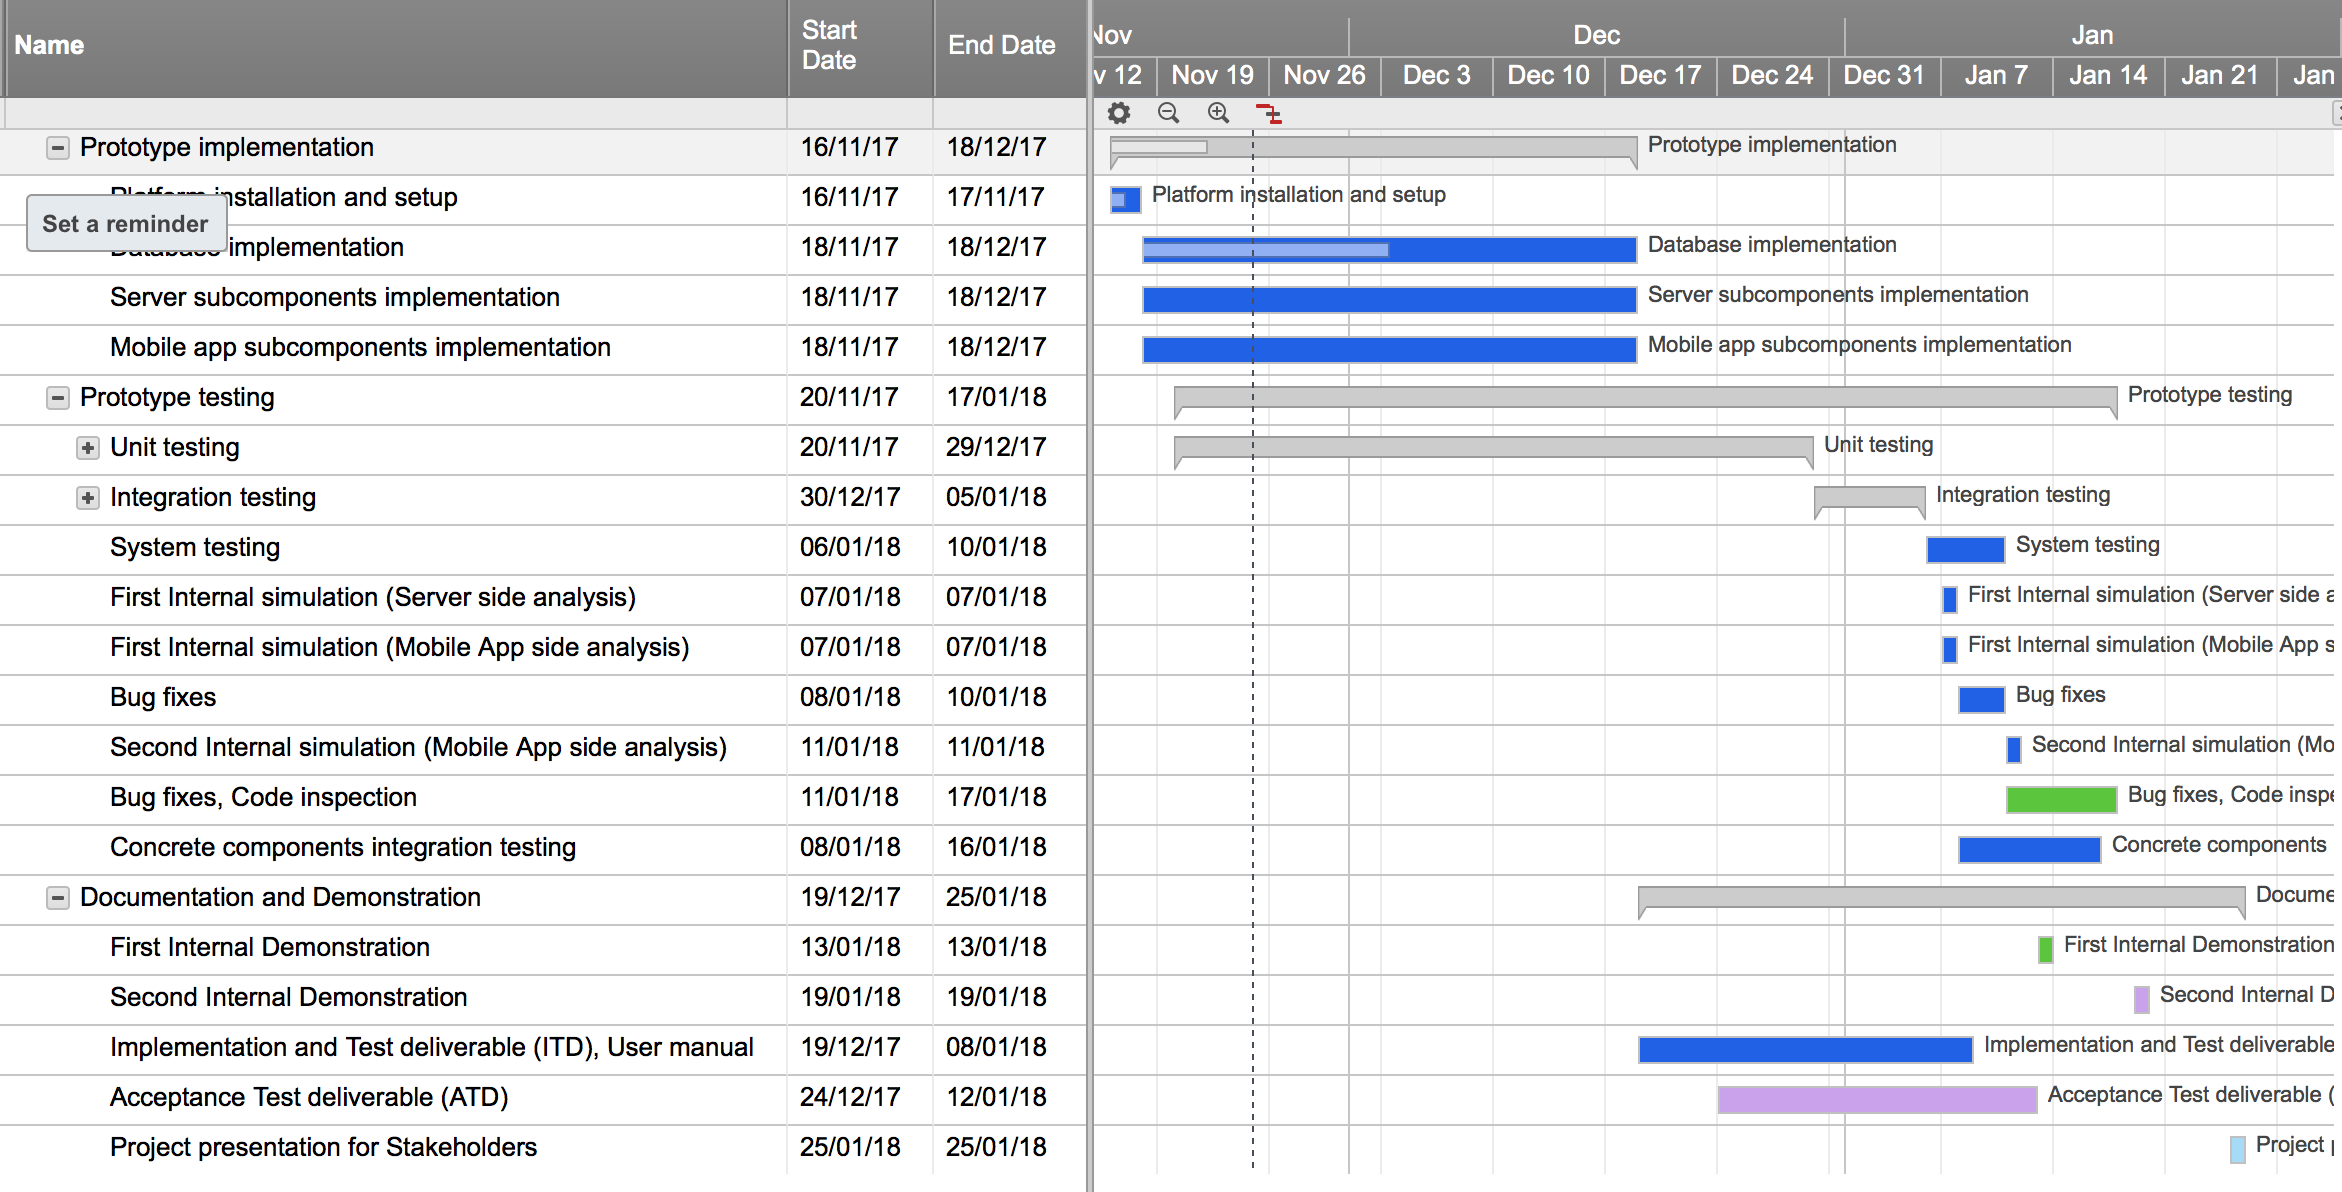
\includegraphics[scale=0.3]{Guantt_diagram_25112017_1}
	\end{centering}
	\caption{Guantt diagram for implementation schedule}
\end{figure}

\newpage
\subsection{Integration and test}

\subsubsection{Entry criteria}
In order to begin the integration phase, the following assumptions must be valid:

\begin{itemize}
	\item The RASD and the previous sections of DD must be complete and correct
	\item The database must be complete, configured and operating
	\item The APIs of external companies collaborating with the system must be usable
	\item The classes of the model and their main functionalities have been implememnted and tested, as described in the previous sections.
\end{itemize}

\subsubsection{Integration testing strategy}
We plan to integrate the components incrementally, as soon as they have been implemented and unit tested. As for the implementation, we plan to adopt a mainly bottom up strategy, although it doesn't have to be strictly followed and small changes to this approach can be made, when needed.
We also plan to adopt a critical module approach, testing first the modules which perform the main functionalities of the system.

\subsubsection{Sequence of integration}
As stated in the previous subsection, we will test the main functionalities of the system as soon as possible, which are the creation of meetings and the computation of trips. The communication with external companies is considered a critical operation as well, as it is fundamental for the computation of trips and therefore the creation of meetings.\\
We will first focus on the integration of all components of the server within each other and, once this phase is complete, we will proceed with the integration with the external server, the database and, finally, the user.\\



\begin{enumerate}
	\item BreakController --> Model\\
	      NavigatorController --> Model
	\item TripController --> BreakController, NavigationController, Model
	\item MeetingController --> Model
	\item PathRestrictionController, NotificationManagerController, MeanOfTransportController --> Model
	\item ExternalCompanyController --> PathRestrictionController, NotificationManagerController, Model
	\item ExternalMeanOfTransportCompanyController --> NotificationManagerController, MeanOfTransportController, Model
	\item UserDeviceController --> Model
	\item LoginController --> Model
	\item UserPreferencesController --> Model
	\item APIManager --> ExternalCompanyController, ExternalMeanOfTransportCompanyController
	\item UserController --> MeetingController, TripController, UserDeviceController, LoginController, UserPreferencesController, Model
	\item ConnectionHandler --> UserController
\end{enumerate}

At this point, all the elements of the server will be integrated.
\begin{enumerate}
	\item ExternalServers --> APIManager
	\item Model --> GMSGateway, PushGateway
	\item Model --> Database
	\item User's MobileApp --> ConnectionHandler
\end{enumerate}

\subsubsection{Integration test cases}

\paragraph{Test case IS1.T1}
\begin{itemize}
	\item Test items: BreakController -> Model
	\item Input specifications: break creation request from the TripController
	\item Output specifications: a new Break is correctly created
	\item Description/purpose: the BreakController sends to the Model the specifications about the break the user wants to create. The model sends back the confirm of the creation, or an error message in case the break was unfeasible.
	\item Dependencies: TripController driver
\end{itemize}

\paragraph{Test case IS1.T2}
\begin{itemize}
	\item Test items: NavigatorController -> Model
	\item Input specifications: the user selects a trip to add to his route
	\item Output specifications: the trip is correctly added in the model
	\item Description/purpose: the NavigatorController receives from the TripController the request from a user to select a trip among proposed ones. The selected trip in the navigator is updated and the Model notifies the NavigatorController
	\item Dependencies: TripController driver
\end{itemize}

\paragraph{Test case IS2.T1}
\begin{itemize}
	\item Test items: TripController -> BreakController
	\item Input specifications:
	\item Output specifications:
	\item Description/purpose:
	\item Dependencies: TripController driver
\end{itemize}

\paragraph{Test case IS2.T2}
\begin{itemize}
	\item Test items: TripController -> NavigatorController
	\item Input specifications:
	\item Output specifications:
	\item Description/purpose
	\item Dependencies:
\end{itemize}

\paragraph{Test case IS2.T3}
\begin{itemize}
	\item Test items: TripController -> Model
	\item Input specifications: 
	\item Output specifications: 
	\item Description/purpose
	\item Dependencies:
\end{itemize}

\paragraph{Test case IS3.T1}
\begin{itemize}
	\item Test items: MeetingController -> Model
	\item Input specifications: a meeting creation request is forwarded by the UserController
	\item Output specifications: a new meeting is correctly scheduled
	\item Description/purpose: the MeetingController sends to the Model the specifications about the meeting the user wants to create. The Model sends back the confirm of the meeting creation, or an error message in case it was unfeasible
	\item Dependencies: UserController driver
\end{itemize}

\paragraph{Test case IS4.T1}
\begin{itemize}
	\item Test items: PathRestrictionController -> Model
	\item Input specifications:
	\item Output specifications:
	\item Description/purpose
	\item Dependencies:
\end{itemize}

\paragraph{Test case IS4.T2}
\begin{itemize}
	\item Test items: NotificationManagerController -> Model
	\item Input specifications:
	\item Output specifications:
	\item Description/purpose
	\item Dependencies:
\end{itemize}

\paragraph{Test case IS4.T3}
\begin{itemize}
	\item Test items: MeanOftransportController -> Model
	\item Input specifications:
	\item Output specifications:
	\item Description/purpose
	\item Dependencies:
\end{itemize}

\paragraph{Test case IS5.T1}
\begin{itemize}
	\item Test items: ExternalCompanyController -> PathRestrictionController
	\item Input specifications:
	\item Output specifications:
	\item Description/purpose
	\item Dependencies:
\end{itemize}

\paragraph{Test case IS5.T2}
\begin{itemize}
	\item Test items: ExternalCompanyController -> NotificationManagerController
	\item Input specifications: a notification about bad weather conditions comes from an external company 
	\item Output specifications: the message is correctly handled from the ExternalCompanyController to the NotificationManager
	\item Description/purpose: this test case is an important step in the correct communication with external companies in case a problem that may affect the computation of routes occurs (for example bad weather conditions)
	\item Dependencies: APIManager driver
\end{itemize}

\paragraph{Test case IS5.T3}
\begin{itemize}
	\item Test items: ExternalCompanyController -> Model
	\item Input specifications:
	\item Output specifications:
	\item Description/purpose
	\item Dependencies:
\end{itemize}

\paragraph{Test case IS6.T1}
\begin{itemize}
	\item Test items: ExternalMeanOfTransportCompanyController -> NotificationManagerController
	\item Input specifications: a notification about a strike comes from an external company 
	\item Output specifications: the message is correctly handled from the ExternalMeanOfTransportCompanyController to the NotificationManager
	\item Description/purpose: like test case IS5.T1, this test case is an important step in the correct communication with external companies in case a problem that may affect the computation of routes occurs
	\item Dependencies: APIManager driver
\end{itemize}

\paragraph{Test case IS6.T2}
\begin{itemize}
	\item Test items: ExternalMeanOfTransportCompanyController -> MeanOfTRansportController
	\item Input specifications:
	\item Output specifications:
	\item Description/purpose
	\item Dependencies:
\end{itemize}

\paragraph{Test case IS6.T3}
\begin{itemize}
	\item Test items: ExternalMeanOfTransportCompanyController -> Model
	\item Input specifications:
	\item Output specifications:
	\item Description/purpose
	\item Dependencies:
\end{itemize}

\paragraph{Test case IS7.T1}
\begin{itemize}
	\item Test items: UserDeviceController -> Model
	\item Input specifications:
	\item Output specifications:
	\item Description/purpose
	\item Dependencies:
\end{itemize}


\paragraph{Test case IS8.T1}
\begin{itemize}
	\item Test items: LoginController -> Model
	\item Input specifications: a login request from the user is forwarded from the UserController
	\item Output specifications: the user is granted access to his account, or denied if wrong data was inserted
	\item Description/purpose: this test case is important for granting the security of users' data
	\item Dependencies: Database stub, UserController driver
\end{itemize}

\paragraph{Test case IS9}
\begin{itemize}
	\item Test items: UserPreferencesController -> Model
	\item Input specifications: a request from the user to set the trip's preferences is forwarded from the UserController
	\item Output specifications: preferences are correctly set
	\item Description/purpose: this case tests the functionality of allowing the setting of preferences and constraints for a route, for example preferable or unwanted travel means
	\item Dependencies: UserController device
\end{itemize}

\paragraph{Test case IS10.T1}
\begin{itemize}
	\item Test items: APIManager -> ExternalCompanyController
	\item Input specifications: request of maps from an external company for the trip computation
	\item Output specifications: the request is correctly sent to the APIManager (and then to external servers) and the maps are sent back
	\item Description/purpose: test the correct interaction with external companies' servers
	\item Dependencies: External server driver, Model stub
\end{itemize}

\paragraph{Test case IS10.T2}
\begin{itemize}
	\item Test items: APIManager -> ExternalMeanOfTransportCompanyController
	\item Input specifications:the user has selected the online purchase of a public transport ticket
	\item Output specifications: redirection to the right company's site
	\item Description/purpose: test the correct interaction with external mean of transport companies' servers
	\item Dependencies: Model stub, External server driver
\end{itemize}

\paragraph{Test case IS11.T1}
\begin{itemize}
	\item Test items: UserController -> MeetingController
	\item Input specifications: incoming message involving meeting
	\item Output specifications: the message is correctly sorted into the MeetingController
	\item Description/purpose: test the correct sorting of incoming messages
	\item Dependencies: ConnectionHandler driver
\end{itemize}

\paragraph{Test case IS11.T2}
\begin{itemize}
	\item Test items: UserController -> TripController
	\item Input specifications: incoming message involving trip
	\item Output specifications: the message is correctly sorted into the TripController
	\item Description/purpose: test the correct sorting of incoming messages
	\item Dependencies: ConnectionHandler driver
\end{itemize}

\paragraph{Test case IS11.T3}
\begin{itemize}
	\item Test items: UserController -> UserDeviceController
	\item Input specifications: incoming message involving ???
	\item Output specifications: the message is correctly sorted into the UserDeviceController
	\item Description/purpose: test the correct sorting of incoming messages
	\item Dependencies: ConnectionHandler driver 
\end{itemize}

\paragraph{Test case IS11.T4}
\begin{itemize}
	\item Test items: UserController -> LoginController
	\item Input specifications: incoming message involving access or registration
	\item Output specifications: the message is correctly sorted into the LoginController
	\item Description/purpose: test the correct sorting of incoming messages
	\item Dependencies: ConnectionHandler driver
\end{itemize}

\paragraph{Test case IS11.T5}
\begin{itemize}
	\item Test items: UserController -> UserPreferencesController
	\item Input specifications: incoming message involving user's preferences
	\item Output specifications: the message is correctly sorted into the UserPreferencesController
\item Description/purpose: test the correct sorting of incoming messages
\item Dependencies: ConnectionHandler driver 
\end{itemize}

\paragraph{Test case IS12.T1}
\begin{itemize}
	\item Test items: ConnectionHandler -> UserController
	\item Input specifications: a message from the user's Mobile Application reaches the ConnectionHandler
	\item Output specifications: the message is correctly handled from the ConnectionHandler to the UserController
	\item Description/purpose: test the correct communication between the reception of messages from the Mobile Application and the components that sortes them to the right controller
	\item Dependencies: none
\end{itemize}

\newpage
\section{Effort spent}
\subsection{Bolshakova Liubov}
\begin{itemize}
	\item 
\end{itemize}
\subsection{Campagnoli Chiara}
\begin{itemize}
	\item 
\end{itemize}
\subsection{Lagni Luca}
\begin{itemize}
	\item 
\end{itemize}

%\newpage
%\section{References}
	
\end{document}